% siminos/presentations/kittens/Rutgers20.tex  pdflatex Rutgers20; biber Rutgers20
% $Author: predrag $ $Date: 2020-10-09 16:56:44 -0500 (Fri, 09 Oct 2020) $

% FROZEN                                                    2020-12-16

%  lectures/QFT20/ kittens.pdf saved as                     2020-09-27
%          ChaosBook.org/overheads/spatiotemporal/QFT20.pdf
%  started with siminos/presentations/GTmath18/GTmath18.tex 2018-03-02
%  started with siminos/presentations/KITP17/UCSB17.tex     2017-01-26
%  started with siminos/presentations/Israel16/Israel16.tex 2016-08-17
%  started with siminos/presentations/GTmap16/GTmap16.tex   2016-08-17
%  started with talks/predrag/NBI16/NBI16.tex               2016-04-25
%  started with talks/predrag/RoySoc16/RoySoc16.tex         2016-04-25

                        \newif\ifboyscout\boyscouttrue          %% comments     %%
                        \newif\ifsubmission\submissionfalse     %% internal     %%
                        \newif\ifblog\blogfalse %% section shared with blogCats %%

\input ../../inputs/layoutBeamer
\usepackage[font=scriptsize, labelfont=bf]{caption}
\usepackage[
    backend=biber,  %bibtex,
    sorting=nyt,
    %refsection=chapter,
    %citereset=chapter,
    style=numeric, %alphabetic, % %style=authoryear,
    natbib=true,
    style=phys, % aps
    biblabel= brackets, % superscript, %
    articletitle=false, % true,  % false, % aps
    %chaptertitle=true,  % aip;  % false, % aps
    pageranges = true , % aip: the full range
             % = false, % aps: only the first page being printed
    sortlocale=en_US,
    firstinits=true,
    url=false, %true,  %
    doi=false, %true,
    eprint=false
]{biblatex}
\addbibresource{../../bibtex/siminos.bib}
\setbeamerfont{footnote}{size=\tiny}
%\input ../../inputs/def % no edits, always from dasbuch/book/inputs
\input defsKittens
\input ../../inputs/defsBeamer
\renewcommand{\Ssym}[1]{{\ensuremath{m_{#1}}}}    % Boris
% \newcommand{\Ssym}[1]{{\ensuremath{s_{#1}}}}  % ChaosBook
% \newcommand{\D}{\mathcal{D}}
% \newcommand{\gd}{\mathsf{g}}

\begin{document}
\title{
{\huge \catlatt}
    \\
{a chaotic field theory}
}
\author{P. Cvitanovi\'c}
\author[Cvitanovi\'c]
{
  \textcolor{green!50!black}{
  {Predrag~Cvitanovi\'c
    and
    Han Liang
%   \\
%  Matt Gudorf,
  }	%\inst{1}
  }
}
\institute
{
                    {\large Georgia Tech}
\\
%  \inst{1}%
%\HREF{https://itsatcuny.org/calendar/chaos-and-quantum-field-theory}
%{Rutgers Mathematical Physics Seminar}
\HREF{http://ChaosBook.org/overheads/spatiotemporal}
 {ChaosBook.org/overheads/spatiotemporal}
 \\ \bigskip
             Mathematical Physics Pandeminar\\
                Rutgers University
 }
\date{December 16, 2020}

\begin{frame}
  \titlepage
\end{frame}

\begin{frame}{Q. what is a chaotic field theory?}
    \begin{block}{A. say it three times}
{\textcolor{blue}{Bernoulli coin flip}}
\bigskip

\hfill serves here is the stage 1 of an introduction to the

{\textcolor{blue}{\catlatt}\footfullcite{CL18}}
\bigskip

\hfill which is the simplest example of % the larger picture

 \textcolor{blue}{spatiotemporally chaotic field theory}\footfullcite{GuBuCv17}
\bigskip\bigskip\bigskip
    \end{block}
\end{frame} %%%%%%%%%%%%%%%%%%%%%%%%%%%%%%%%%%%%%%%%%%%%%%


\begin{frame}{a motivation : need a theory of {\Huge large} fluid domains}
pipe flow close to onset of turbulence
\footnote{M.~Avila and B.~Hof, {Phys. Rev. \bf E 87} (2013)}
\begin{center}
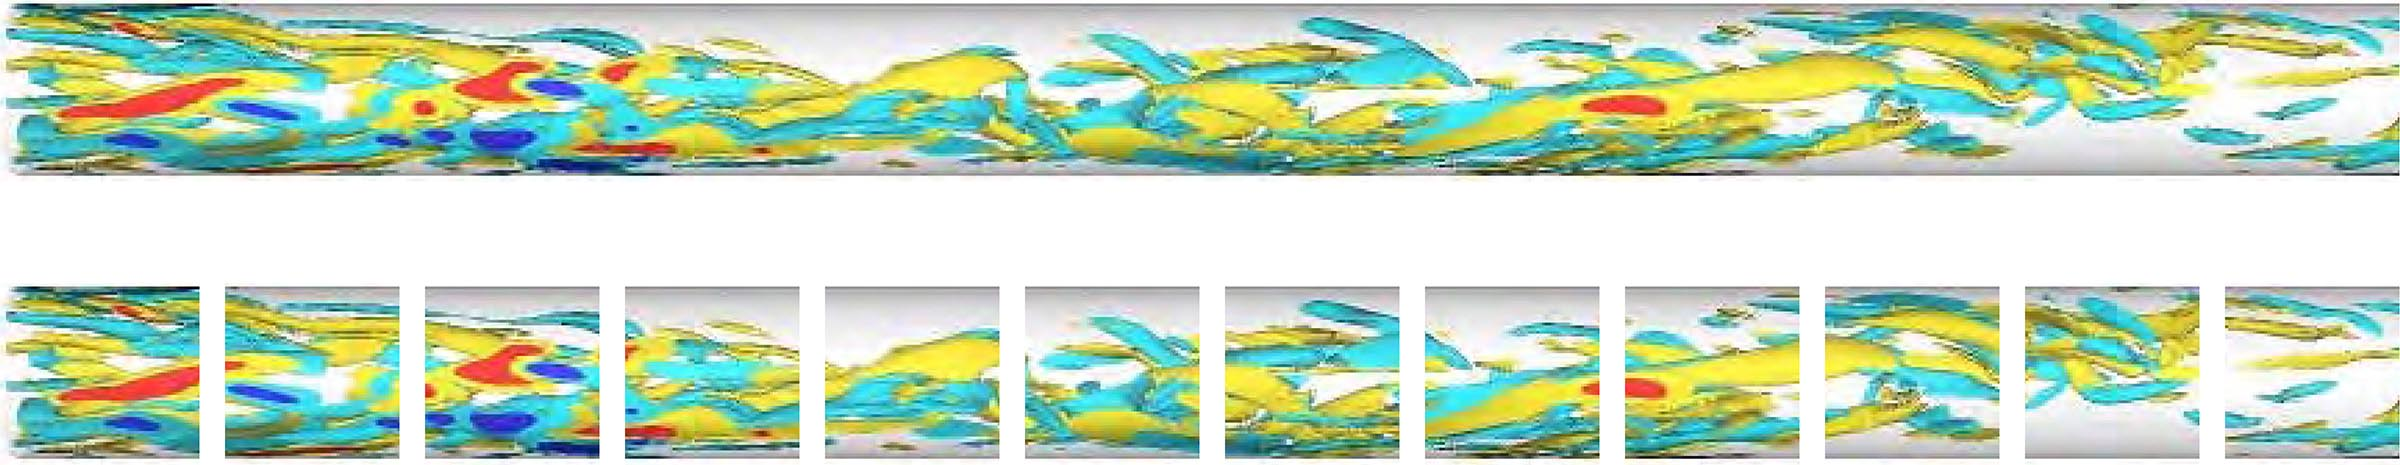
\includegraphics[width=1.0\textwidth]{AviHof13fig4CLM}
\end{center}
we have a detailed theory of {\small \textcolor{blue}{small}} turbulent fluid cells

\bigskip

can we can we construct the \textcolor{red}{infinite} pipe by coupling small turbulent cells ?
\bigskip

\textcolor{blue}{what would that theory look like ?}
\end{frame} %%%%%%%%%%%%%%%%%%%%%%%%%%%%%%%%%%%%%%%%%%%%%%


\begin{frame}{the goal}
\vfill

\begin{center}
{\Large build
\\
a \textcolor{blue}{chaotic field theory}
\medskip

from
\\
the simplest \textcolor{blue}{chaotic blocks}
}
\end{center}

\vfill
using
\begin{itemize}
  \item
\textcolor{blue}{time invariance}
  \item
\textcolor{blue}{space invariance}
\end{itemize}
 of the defining partial differential equations
\end{frame} %%%%%%%%%%%%%%%%%%%%%%%%%%%%%%%%%%%%%%%%%%%%%%

\begin{frame}{take-home :   }
\begin{center}
            \begin{minipage}[c]{0.40\textwidth}\begin{center}
{\color{purple}harmonic} field theory
\bigskip

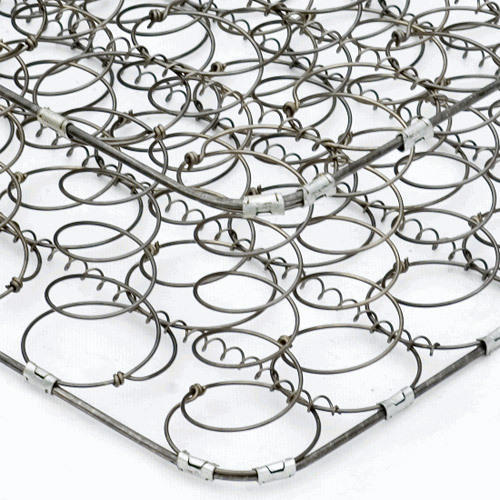
\includegraphics[width=0.85\textwidth]{mattressSpring}\\
{\color{blue}tight-binding} model \\ ({\color{blue}Helmholtz})
            \end{center}\end{minipage}
            \hspace{2ex}
            \begin{minipage}[c]{0.46\textwidth}\begin{center}
{\color{purple}chaotic} field theory\\
\bigskip
\bigskip
\bigskip

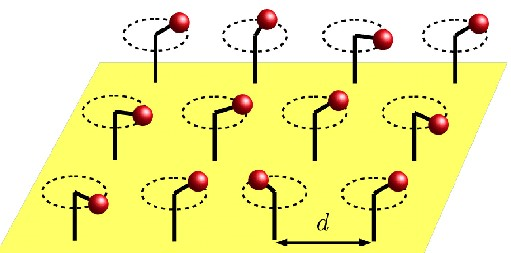
\includegraphics[width=1.0\textwidth]{flagellum1}\\
\bigskip

Euclidean {\color{blue}Klein-Gordon} \\ (damped {\color{blue}Poisson})
            \end{center}\end{minipage}
\end{center}
\end{frame}%%%%%%%%%%%%%%%%%%%%%%%%%%%%%%%%%%%%%%%%%%%%%%

\begin{frame}{take-home :   }
\begin{center}
            \begin{minipage}[c]{0.40\textwidth}\begin{center}
{\color{purple}harmonic} field theory
\bigskip

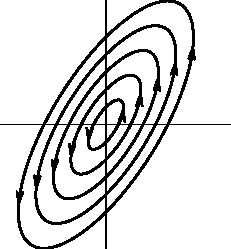
\includegraphics[width=0.35\textheight]{twodlinearEll}\\
\bigskip

{\color{blue}oscillatory eigenmodes}
            \end{center}\end{minipage}
            \hspace{2ex}
            \begin{minipage}[c]{0.46\textwidth}\begin{center}
{\color{purple}chaotic} field theory\\
\bigskip

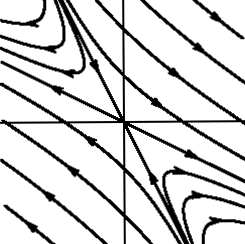
\includegraphics[width=0.35\textheight]{twodlinearHyp}\\
\bigskip

{\color{blue}hyperbolic instabilities}
            \end{center}\end{minipage}
\end{center}
\end{frame} %%%%%%%%%%%%%%%%%%%%%%%%%%%%%%%%%%%%%%%%%%%%%%

\section[a coin toss]
 {a coin toss}

\begin{frame}{}
\begin{bartlett}{
Mephistopheles knocks at Faust's door and says, ``Du
mu{\ss}t es dreimal sagen!"
\\{\color{yellow}.}\qquad
{\scriptsize\emph{``You have to say it three times"}}
        }
\bauthor{
Johann Wolfgang von Goethe
\\{\color{yellow}.}\qquad\quad
{\em Faust I - Studierzimmer 2.~Teil}%\rf{GoetheIstuZim1806}
    }
\end{bartlett}
\vfill
\begin{enumerate}
%              \item \textcolor{gray}{\small
%what this is about
%                  }
              \item {\Large
coin toss
                  }\textcolor{gray}{\small
              \item
\templatt
              \item
\catlatt
              \item
bye bye, dynamics
                    }
            \end{enumerate}
\end{frame}

\renewcommand{\ssp}{\ensuremath{x}}               % state space point

\begin{frame}{(1)  coin toss, traditional}
\vfill
    \begin{center}
{\huge time-evolution formulation}
    \end{center}
\vfill
\end{frame} %%%%%%%%%%%%%%%%%%%%%%%%%%%%%%%%%%%%%%%%%%%%%%

\begin{frame}{fair coin toss} % ~~~(AKA  }
\renewcommand{\ssp}{\ensuremath{\phi}}             % lattice site field
    \begin{block}{{Bernoulli}  map} %the essence of deterministic chaos}
\begin{center}
            \begin{minipage}[c]{0.36\textwidth}\begin{center}
% ChaosBook {fig:BernPartExam}
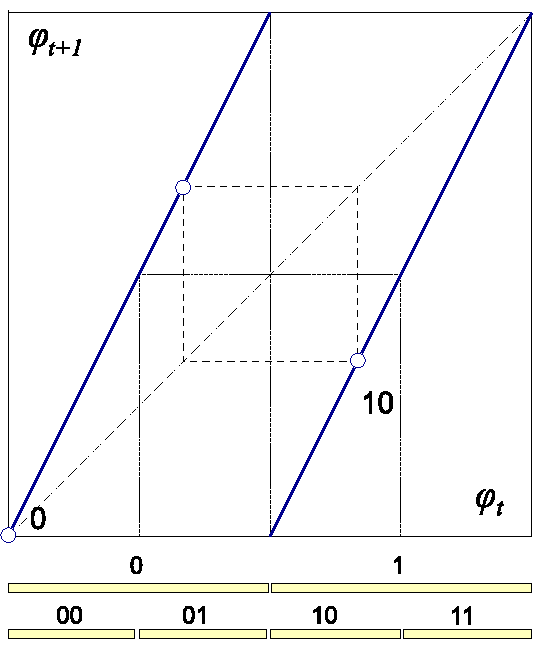
\includegraphics[width=1.0\textwidth]{BernPartKitten}
            \end{center}\end{minipage}
            \hspace{2ex}
            \begin{minipage}[c]{0.46\textwidth}\begin{center}
\[
\ssp_{\zeit+1} =
% \flow{}{\ssp_{\zeit}} =
\left\{ \begin{array}{l} %l}
        % f_0(\ssp_{\zeit}) =
        2 \ssp_{\zeit}
                             \\% \,, \quad & \ssp_{\zeit} \in \pS_0=[0,1/2) \\
        % f_1(\ssp_{\zeit}) =
        2 \ssp_{\zeit} \;\; (\mbox{mod}\;1)
                             % \,, \quad       & \ssp_{\zeit} \in \pS_1 =[1/2,1)
         \end{array}\right.
\]
            \end{center}\end{minipage}
\end{center}
%$\cl{}=2$ and 4 intervals \statesp\ partitions,

\hfill $\Rightarrow$~~~~~
fixed point \cycle{0}, 2-cycle \cycle{01}, $\cdots$
    \end{block}

\bigskip

a \HREF{https://www.random.org/coins/?num=2&cur=40-antique.aurelian}
{coin toss}

\hfill the essence of {\color{blue}deterministic chaos}
\end{frame} %%%%%%%%%%%%%%%%%%%%%%%%%%%%%%%%%%%%%%%%%%%%%%

\begin{frame}{what is ({mod}\;1) ?}
\renewcommand{\ssp}{\ensuremath{x}}             % lattice site field
map with integer-valued {\color{blue}`stretching' parameter $s\geq2$} :
\[
\ssp_{\zeit+1} \,=\, {s}\,\ssp_{\zeit}
\] %ee{BerStretch}

$(\mbox{mod}\;1)$ :
subtract the integer part
\(
\Ssym{\zeit+1}=\left\lfloor{s}\ssp_{\zeit}\right\rfloor
\)

\renewcommand{\ssp}{\ensuremath{\phi}}             % lattice site field
so fractional part
$\ssp_{\zeit+1}$ stays in the unit interval $[0,1)$
\[
\ssp_{\zeit+1}
= {s} \ssp_{\zeit} - \Ssym{\zeit+1}
\,,\qquad  \ssp_{\zeit}\in\pS_{\Ssym{\zeit}}
\] %ee{circ-m}
$\Ssym{\zeit}$ takes values in the ${s}$-letter alphabet
\[
\Ssym{} \in \A=\{0,1,2,\cdots,s-1\}
\] %ee{base-sAlph}
\end{frame} %%%%%%%%%%%%%%%%%%%%%%%%%%%%%%%%%%%%%%%%%%%%%%

\renewcommand{\ssp}{\ensuremath{\phi}}             % lattice site field

\begin{frame}{a fair dice throw}
    \begin{block}{slope ${6}$ Bernoulli map}
\begin{center}
            \begin{minipage}[c]{0.32\textwidth}\begin{center}
% ChaosBook {fig:BernPartExam}
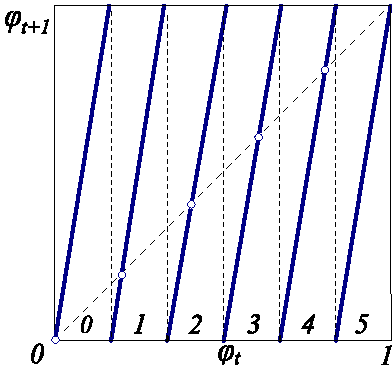
\includegraphics[width=1.0\textwidth]{fig_d_2kitten} % {fig_d_2CL18}
            \end{center}\end{minipage}
            \hspace{2ex}
            \begin{minipage}[c]{0.46\textwidth}
\(
\ssp_{\zeit+1}
= {6} \ssp_{\zeit} - \Ssym{\zeit+1}
\,,\;  \ssp_{\zeit}\in\pS_{\Ssym{\zeit}}
\)
\medskip

${6}$-letter alphabet \\
\(
\Ssym{\zeit} \in \A=\{0,1,2,\cdots,5\}
\)
            \end{minipage}
\end{center}
$6$ subintervals $\{\pS_{0},\pS_{1},\cdots,\pS_{5}\}$
    \end{block}
\end{frame} %%%%%%%%%%%%%%%%%%%%%%%%%%%%%%%%%%%%%%%%%%%%%%

\begin{frame}{what is chaos ?}
    \begin{block}{a fair dice throw}
$6$ subintervals $\{\pS_{\Ssym{\zeit}}\}$,
$6^2$ subintervals $\{\pS_{\Ssym{1}\Ssym{2}}\}, \cdots$
\begin{center}
            \begin{minipage}[c]{0.32\textwidth}\begin{center}
% ChaosBook {fig:BernPartExam}
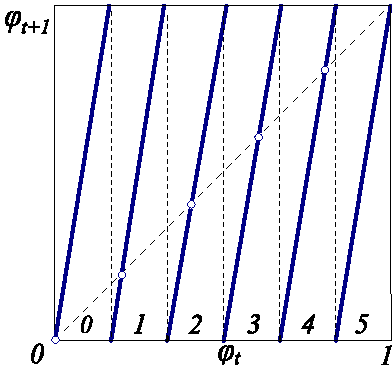
\includegraphics[width=1.0\textwidth]{fig_d_2kitten} % {fig_d_2CL18}
            \end{center}\end{minipage}
            \hspace{2ex}
            \begin{minipage}[c]{0.46\textwidth}
each subinterval contains a periodic point,
labeled by
$\Mm=\Ssym{1}\Ssym{2}\cdots\Ssym{\cl{}}$
\bigskip

$N_\cl{} = 6^\cl{}$ {\color{red}unstable} orbits
            \end{minipage}
\end{center}
    \end{block}
\vfill
    \begin{block}{definition : chaos is}
positive Lyapunov $(\ln s)$ - positive entropy $(\frac{1}{\cl{}}\ln N_\cl{})$
    \end{block}
\end{frame} %%%%%%%%%%%%%%%%%%%%%%%%%%%%%%%%%%%%%%%%%%%%%%

\begin{frame}{}
    \begin{block}{definition : chaos is}
positive {\color{blue}Lyapunov} $(\ln s)$
         -
positive {\color{blue}entropy} $(\frac{1}{\cl{}}\ln N_\cl{})$
    \end{block}
\bigskip
\begin{itemize}
  \item {\color{blue}Lyapunov} : how fast is local escape?
  \item {\color{blue}entropy} ~~~: how many ways of getting back?
\end{itemize}
                \hfill $\Rightarrow$ {\color{blue}ergodicity}
\vfill
%\hfill
the precise sense in which
\HREF{https://www.random.org/dice/}{dice throw}\\
is an example of deterministic chaos
\end{frame} %%%%%%%%%%%%%%%%%%%%%%%%%%%%%%%%%%%%%%%%%%%%%%

\begin{frame}{(2) chaos for field theorists, 3rd millenium}
\vfill
\begin{center}
{\huge lattice formulation}
\end{center}
\vfill
\end{frame} %%%%%%%%%%%%%%%%%%%%%%%%%%%%%%%%%%%%%%%%%%%%%%

\renewcommand{\Xx}{\ensuremath{\Phi}}

\begin{frame}{lattice Bernoulli}
recast the time-evolution Bernoulli map
\[
\ssp_{\zeit+1}
= {s} \ssp_{\zeit} - \Ssym{\zeit+1}
\] %ee{circ-m}
as 1-step difference equation on the {\color{blue}temporal lattice}
\beq
\ssp_{\zeit} - {s}\ssp_{\zeit-1} = - \Ssym{\zeit}
\,,\qquad  \ssp_{\zeit} \in [0,1)
\ee{1stepDiffEq}
{\color{blue}field} $\ssp_\zeit$, {\color{blue}source} $\Ssym{\zeit}$ \\
on each site $\zeit$ of a
1\dmn\ lattice $\zeit\in\integers$
\bigskip

 write an \cl{}-sites lattice segment as \\
the {\color{blue}lattice state} and the {\color{blue}symbol \brick}
\beq
{\Xx} % = \{\ssp_j\}
             = (\ssp_{\zeit+1},\cdots,\ssp_{\zeit+\cl{}})
\,,\quad
{\Mm} % = \{\Ssym{j}\}
             = (\Ssym{{\zeit+1}},\cdots,\Ssym{{\zeit+\cl{}}})
\ee{pathBern}
`$\Mm$' for `marching orders' ~~:~~ come here, then go there, $\cdots$
\end{frame} %%%%%%%%%%%%%%%%%%%%%%%%%%%%%%%%%%%%%%%%%%%%%%

\begin{frame}{exponentially many distinct walks through Bernoullistan}
\begin{center}
\hfill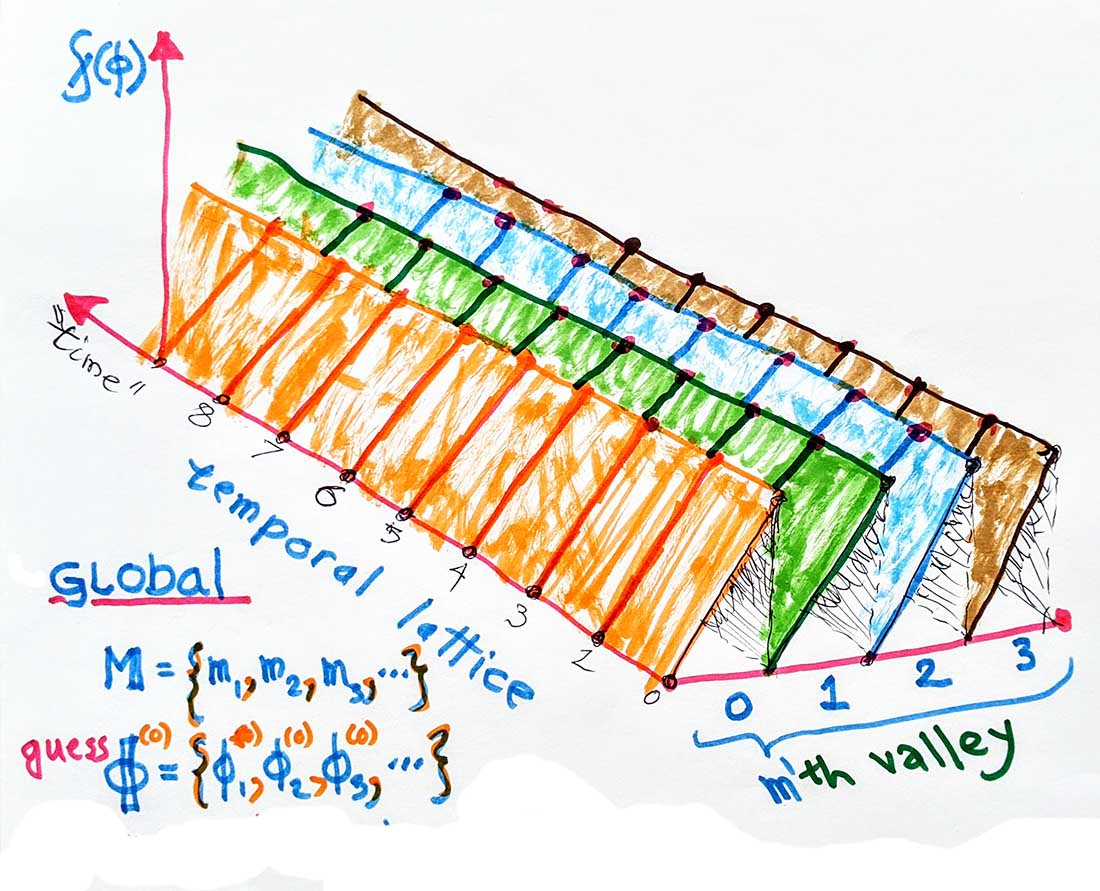
\includegraphics[width=0.90\textwidth]{PC200923Bernoulli1}
\end{center}
\end{frame} %%%%%%%%%%%%%%%%%%%%%%%%%%%%%%%%%%%%%%%%%%%%%%


\begin{frame}{think globally, act locally}
Bernoulli {\color{blue}condition} at every lattice site $\zeit$,
{\color{blue}local} in time
\beq
\ssp_{\zeit} - {s}\ssp_{\zeit-1} = - \Ssym{\zeit}
\ee{1stepDiffEq}
is enforced by the {\color{blue}global} equation
\beq
\left(\unit-{s}\,\hopMat^{-1}\right)\,\Xx = - \Mm
\,,
\ee{tempBern}
$[\cl{}\!\times\!\cl{}]$ shift matrix
\beq
\hopMat_{jk}=\delta_{j+1,k}
\,,\qquad
\hopMat
=  \left(\begin{array}{ccccc}
             0    &  1    &        &   &  \cr
                  &  0    &   1    &   &  \cr
                  &       &        & \ddots &  \cr
                  &       &        & 0 & 1 \cr
             1    &       &        &   & 0
          \end{array} \right)
\ee{hopMatrix}
compares the neighbors
\end{frame} %%%%%%%%%%%%%%%%%%%%%%%%%%%%%%%%%%%%%%%%%%%%%%

\begin{frame}{think globally, act locally}
solving the {lattice Bernoulli} system
\[
\jMorb\Xx= -\Mm
\,,
\]
$[\cl{}\!\times\!\cl{}]$ {\color{blue}Hill matrix}
~~~~~~~~~~~~~~~
\(
\jMorb = \unit-{s}\,{\hopMat}^{-1}
\,,
\) %{tempBernFix}
\medskip

is a search for zeros of the function
\beq
F[\Xx] = \jMorb\Xx+\Mm = 0
\ee{tempFixPoint}
the entire {\color{blue}global lattice state} ${\Xx}_{\Mm}$ is now
\medskip

a single {\color{blue}fixed point}
$(\ssp_1,\ssp_{2},\cdots,\ssp_{\cl{}})$

\hfill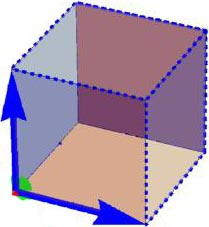
\includegraphics[width=0.12\textwidth]{hyperCube}

\hfill
in the \cl{}\dmn\ unit hyper-cube ~~~~~~~~~~~$\Xx\in[0,1)^\cl{}$
\end{frame} %%%%%%%%%%%%%%%%%%%%%%%%%%%%%%%%%%%%%%%%%%%%%%

\begin{frame}{\jacobianOrb}
solving a nonlinear
\[
F[\Xx]=0 \quad \mbox{ \color{blue}fixed point condition}
\]
with Newton method requires evaluation of
the $[\cl{}\!\times\!\cl{}]$
    \begin{block}{\jacobianOrb}
\[
\jMorb_{ij} =\frac{\delta F[\Xx]_i}{\delta \ssp_j}
\] %ee{jacobianOrb}
    \end{block}

what does this global \jacobianOrb\ do?
\bigskip

\begin{enumerate}
              \item
fundamental fact {\color{red}!}
              \item
global stability of lattice state \Xx, perturbed everywhere
            \end{enumerate}
\end{frame} %%%%%%%%%%%%%%%%%%%%%%%%%%%%%%%%%%%%%%%%%%%%%%

\begin{frame}{(1)}
\vfill
\begin{center}
{\huge fundamental fact}
\end{center}
\vfill
\end{frame} %%%%%%%%%%%%%%%%%%%%%%%%%%%%%%%%%%%%%%%%%%%%%%

\begin{frame}{(1) fundamental fact}
to satisfy the fixed point condition
\[
\jMorb\Xx+\Mm = 0
\]
the
 {\jacobianOrb} \jMorb\
\begin{enumerate}
              \item
stretches the unit hyper-cube $\Xx\in[0,1)^\cl{}$ into the \cl{}\dmn\
{\color{blue}\fundPip}
              \item
maps each periodic point ${\Xx}_{\Mm}\;\;\Rightarrow\;\;$ integer lattice
$\integers^\cl{}$ point
              \item
then translate by integers ~~$\Mm\;\;\Rightarrow\;\;$ into the origin
            \end{enumerate}
hence $N_\cl{} =$ total $\sharp$ solutions ~~=~~ $\sharp$
integer lattice points within the {\fundPip}

\bigskip

the {\color{blue}fundamental fact}\footfullcite{BaHePl97} :
{\color{blue}\HillDet} counts solutions
\[
N_\cl{} = |\Det\jMorb|
\] %ee{detBern0}
$\sharp$ integer points in {\fundPip} $=$ its volume
\end{frame} %%%%%%%%%%%%%%%%%%%%%%%%%%%%%%%%%%%%%%%%%%%%%%

\begin{frame}{example : {\fundPip} for $\cl{}=2$}
%$[2\!\times\!2]$

{\jacobianOrb} for ${s} = 2$ ;
unit square basis vectors ;
their images :
\beq
\jMorb =
 \left(\begin{array}{cc}
  1 & -2 \\
 -2 &  1
 \end{array} \right)
;\quad
\Xx_B =
 \left(\begin{array}{c}
 1  \\
 0
 \end{array} \right)
\;\to\;
\Xx_{B'} = \jMorb\,\Xx_B =
 \left(\begin{array}{c}
  1  \\
 -2
 \end{array} \right)
\cdots\,,
\ee{bernFundPar}
%\medskip

    \begin{block}{Bernoulli periodic points of period 2}
\begin{center}
            \begin{minipage}[c]{0.32\textwidth}\begin{center}
% ChaosBook {fig:BernPartExam} % BernCyc2Jacob.svg
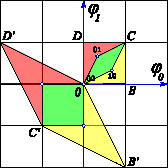
\includegraphics[width=1.0\textwidth]{BernCyc2JacobUnit}
            \end{center}\end{minipage}
            \hspace{2ex}
            \begin{minipage}[c]{0.46\textwidth}
$N_2=3$
\medskip


fixed point ~~$\Xx_{00}$\\
2-cycle ~~~~~~~$\Xx_{01}$, $\Xx_{10}$
            \end{minipage}
\end{center}
    \end{block}
\medskip

square $[0BCD]$
$\Rightarrow\jMorb\Rightarrow$
{\fundPip} $[0B'C'D']$
\end{frame} %%%%%%%%%%%%%%%%%%%%%%%%%%%%%%%%%%%%%%%%%%%%%%

\begin{frame}{fundamental fact for any $\cl{}$}

    \begin{block}{an $\cl{}=3$ example} %{\templatt\ $\cl{}=3$ example}
$\jMorb\,$[unit hyper-cube] = [{\fundPip}]
\begin{center}
            \begin{minipage}[c]{0.32\textwidth}\begin{center}
% ChaosBook {fig:BernPartExam} % BernCyc2Jacob.svg
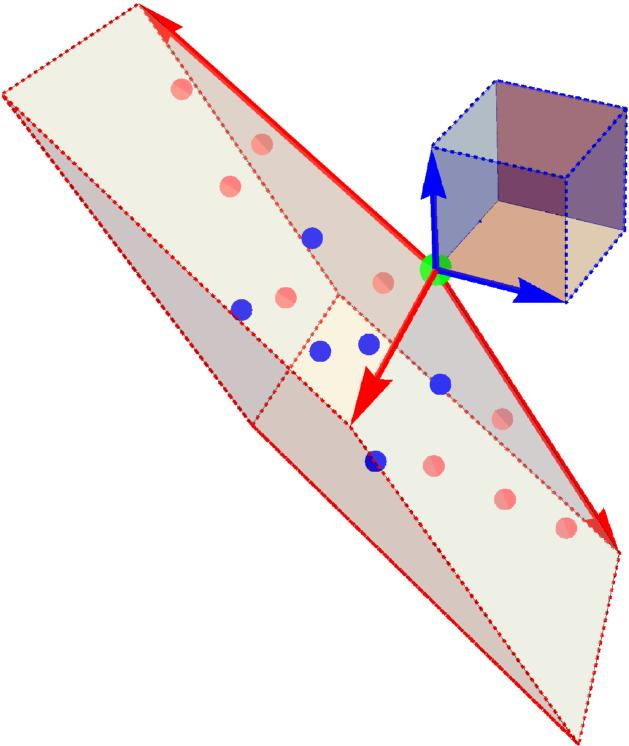
\includegraphics[width=1.0\textwidth]{PCLength3Counting}
            \end{center}\end{minipage}
            \hspace{2ex}
            \begin{minipage}[c]{0.46\textwidth}
unit hyper-cube $\Xx\in[0,1)^3$
\bigskip\bigskip

{\footnotesize $n>3$ cannot visualize}
            \end{minipage}
\end{center}
    \end{block}
    {\footnotesize
a periodic point $\Rightarrow$ integer lattice point :
{\color{red}$\bullet$} on a face,
{\color{blue}$\bullet$} in the interior
    }
\end{frame} %%%%%%%%%%%%%%%%%%%%%%%%%%%%%%%%%%%%%%%%%%%%%%

\begin{frame}{(2)}
\vfill
\begin{center}
{\huge orbit stability}
\end{center}
\vfill
\end{frame} %%%%%%%%%%%%%%%%%%%%%%%%%%%%%%%%%%%%%%%%%%%%%%

\begin{frame}{(2) orbit stability vs. temporal stability}
\begin{block}{\jacobianOrb}
\(
\jMorb_{ij} =\frac{\delta F[\Xx]_i}{\delta \ssp_j}
\)
stability under {\color{blue}global} perturbation of the whole orbit

\hfill for \cl{} large, a huge $[d\cl{}\!\times\!d\cl{}]$ matrix
\end{block}
\begin{block}{temporal {\jacobianM}}
\(
\jMps%_\Mm
\)
propagates {\color{blue}initial} perturbation $\cl{}$ time steps

\hfill small $[d\!\times\!d]$ matrix
\end{block}
\vfill

$\jMps$ and $\jMorb$ are related by\footfullcite{Hill86}
\begin{block}{Hill's 1886 remarkable formula}
\[
|\Det\jMorb_\Mm| = |\det(\matId - \jMps_\Mm)|
%\label{catHillform}
\]
\end{block}
$\jMorb$ is {\color{red}huge}, even $\infty$\dmn\ matrix\\
$\jMps$ is {\color{red}tiny}, few degrees of freedom matrix
\end{frame} %%%%%%%%%%%%%%%%%%%%%%%%%%%%%%%%%%%%%%%%%%%%%%

\begin{frame}{field theorist's chaos}
    \begin{block}{definition : chaos is}
expanding ~~~~~~~~~~~{\color{blue}\HillDet s}
~~~~~~~~~~~$\Det\jMorb$

exponential $\sharp$~~~~~~~~{\color{blue}field configurations}
~~~~~~~$N_\cl{}$~~~
    \end{block}

\bigskip
%\hfill
the precise sense in which

a (discretized) {\color{blue}field theory}
is {\color{blue}deterministically chaotic}

\vfill
 {\color{red}\huge note} : there is no `time' in this definition
\end{frame} %%%%%%%%%%%%%%%%%%%%%%%%%%%%%%%%%%%%%%%%%%%%%%

\begin{frame}{}
\vfill
\begin{center}
{\huge \po\ theory}
\end{center}
\vfill
\end{frame} %%%%%%%%%%%%%%%%%%%%%%%%%%%%%%%%%%%%%%%%%%%%%%

\begin{frame}{volume of a \po}
Ozorio de Almeida and Hannay\footfullcite{OzoHan84} 1984 :\\
$\sharp$ of periodic points is related to a \JacobianM\ by
\begin{block}{principle of uniformity}
``periodic points of an ergodic system, counted with their natural
weighting, are uniformly dense in phase space''
\end{block}
\bigskip

where
\begin{block}{`natural weight' of \po\ {\Mm}}
\[
  \frac{1}{|\det(\unit - \jMps_{\Mm})|}
\]
\end{block}
\end{frame} %%%%%%%%%%%%%%%%%%%%%%%%%%%%%%%%%%%%%%%%%%%%%%

\begin{frame}{\po s partition lattice states into neighborhoods}
how come {\color{blue}\HillDet} $\Det\jMorb$ counts periodic points ?
\bigskip

`principle of uniformity' is in \footfullcite{CBgetused}
\begin{block}{\po\ theory}
known as the \HREF{http://chaosbook.org/chapters/ChaosBook.pdf\#section.27.4} {flow
conservation} sum rule  :
\beq
\sum_{{\Mm}} %\ssp_i{\in\mbox{\footnotesize Fix}\map^{\cl{}}}}
    \frac{1}{|\det (\unit - \jMps_{\Mm})|}
    \;=
\sum_{{\Mm}} %{\ssp_i{\in\mbox{\footnotesize Fix}\map^{\cl{}}}}
    \frac{1}{|\Det\jMorb_{\Mm}|}
    =1
% \label{H-OdeA_mapsOrb}
\eeq
    {\footnotesize
sum over periodic points $\Xx_{\Mm}$ of period \cl{}
    }
\end{block}

\statesp\ is divided into

\hfill
{\color{blue}neighborhoods} of periodic points of period $\cl{}$
\end{frame} %%%%%%%%%%%%%%%%%%%%%%%%%%%%%%%%%%%%%%%%%%%%%%

\begin{frame}{\po\ counting}
how come a $\Det\jMorb$ counts periodic points ?
\bigskip

\begin{block}{flow conservation sum rule :}
\[
\sum_{\ssp_i{\in\mbox{\footnotesize Fix}\map^{\cl{}}}}
    \frac{1}{|\Det\jMorb_i|}
    =1
% \label{H-OdeA_mapsOrb}
\]
\end{block}
\medskip

Bernoulli system `natural weighting' is simple :
\medskip

the determinant
$\Det\jMorb_i=\Det\jMorb$ the same for all periodic points, whose
number thus verifies the {\color{blue}fundamental fact}
\[
N_\cl{} = |\Det\jMorb|
\] %ee{detBern0}

\medskip


\vfill
    \begin{block}{the number of Bernoulli periodic lattice states}
\(
N_{\cl{}} = |\Det\jMorb| = s^{\cl{}} - 1
\) %\ee{noPerPtsBm}
~~~~~~~~for any $\cl{}$
    \end{block}
\end{frame} %%%%%%%%%%%%%%%%%%%%%%%%%%%%%%%%%%%%%%%%%%%%%%

\begin{frame}{remember the fundamental fact?}
    \begin{block}{period 2 example}
\begin{center}
            \begin{minipage}[c]{0.32\textwidth}\begin{center}
% ChaosBook {fig:BernPartExam} % BernCyc2Jacob.svg
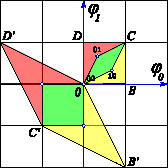
\includegraphics[width=1.0\textwidth]{BernCyc2JacobUnit}
            \end{center}\end{minipage}
            \hspace{2ex}
            \begin{minipage}[c]{0.46\textwidth}
fixed point ~~$\Xx_{00}$\\
2-cycle ~~~~~~~$\Xx_{01}$, $\Xx_{10}$
            \end{minipage}
\end{center}
    \end{block}
\bigskip

$\jMorb\,$[unit hyper-cube] = [{\fundPip}]
\bigskip

look at preimages of the {\fundPip} :
\end{frame} %%%%%%%%%%%%%%%%%%%%%%%%%%%%%%%%%%%%%%%%%%%%%%

\begin{frame}{example : lattice states of period 2}
    \begin{block}{unit hypercube, partitioned}
\begin{center}
            \begin{minipage}[c]{0.32\textwidth}\begin{center}
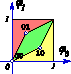
\includegraphics[width=1.0\textwidth]{BernCyc2JacobPart}
            \end{center}\end{minipage}
            \hspace{2ex}
            \begin{minipage}[c]{0.46\textwidth}
fixed point ~~$\Xx_{00}$\\
2-cycle ~~~~~~~$\Xx_{01}$, $\Xx_{10}$
            \end{minipage}
\end{center}
    \end{block}
\medskip

\begin{block}{
\HREF{http://chaosbook.org/chapters/ChaosBook.pdf\#section.27.4} {flow
conservation} sum rule
            }
\beq
      \frac{1}{|\Det{\color{green}\jMorb_{00}}|}
   +    \frac{1}{|\Det{\color{red}\jMorb_{01}}|}
   + \frac{1}{|\Det{\color{yellow}\jMorb_{10}}|}
    =1
% \label{H-OdeA_mapsOrb}
\eeq
    {\footnotesize
sum over periodic points $\Xx_{\Mm}$ of period $\cl{}=2$
    }
\end{block}

\statesp\ is divided into

\hfill
{\color{blue}neighborhoods} of periodic points of period $\cl{}$
\end{frame} %%%%%%%%%%%%%%%%%%%%%%%%%%%%%%%%%%%%%%%%%%%%%%

\begin{frame}{}
\vfill
\begin{center}
{\huge zeta function}
\end{center}
\vfill
\end{frame} %%%%%%%%%%%%%%%%%%%%%%%%%%%%%%%%%%%%%%%%%%%%%%

\begin{frame}{\po\ theory}
how does 1-time step {\color{blue}transition matrix} $T$ count periodic
lattice states ? For any matrix  {\color{blue} $\ln\det=\tr\ln$}, so
\begin{block}{$\ln\det(\unit-zT)=\tr\ln(\unit-zT)\,=\,$ sum over loops}
\[
\det(\unit-zT)= \exp \left(-\sum_{\cl{}=1}\frac{z^\cl{}}{n}\tr T^\cl{}\right)
\]
\end{block}

AKA
\begin{block}{`topological zeta function'}
\[
\zetatop(z)
 \,=\,  \exp \left(-\sum_{\cl{}=1}^\infty
\frac{z^\cl{}}{\cl{}} N_\cl{}
         \right)
\] %label{BernZeta}
\end{block}
        \begin{enumerate}
              \item
weight ${1}/{\cl{}}$
as by (cyclic) translation invariance, $\cl{}$ lattice states are
equivalent
              \item
zeta function counts {\color{blue} prime orbits}, one per each set of equivalent
lattice states
            \end{enumerate}
\end{frame} %%%%%%%%%%%%%%%%%%%%%%%%%%%%%%%%%%%%%%%%%%%%%%

\begin{frame}{Bernoulli \tzeta}
counts {\color{blue}prime orbits},
one per each set of  periodic states $N_\cl{}=s^{\cl{}} - 1$
\[
\zetatop(z)
 \,=\,  \exp \left(-\sum_{\cl{}=1}^\infty
\frac{z^\cl{}}{\cl{}} N_n
         \right)
\,=\,
\frac{1 -  {s}z}{1 - z}
\] %label{BernZeta}
numerator $(1 - {s}z)$ says that Bernoulli orbits are built from \\
$s$
fundamental {\color{blue}primitive} lattice states,

\hfill
the fixed points
$\{\ssp_0,\ssp_1,\cdots,\ssp_{s-1}\}$
\medskip

every other lattice state is
built from their concatenations and repeats.

\vfill
\hfill {\Huge \textcolor{red}{solved!}}
\vfill

{\color{blue}this is `\po\ theory'}
\\
 And if you don't know,
\HREF{https://www.youtube.com/watch?v=_JZom_gVfuw} {now you know}

\end{frame} %%%%%%%%%%%%%%%%%%%%%%%%%%%%%%%%%%%%%%%%%%%%%%

\begin{frame}{think globally, act locally - summary}
\bigskip
the problem of enumerating and determining all global solutions stripped
to its essentials :
\bigskip
\begin{enumerate}
              \item
each solution is a zero of the global {\color{blue}fixed point} condition
\[
F[\Xx] = 0
\]
              \item
{\color{blue}global stability} :  the {\jacobianOrb}
\[
\jMorb_{ij} =\frac{\delta F[\Xx]_i}{\delta \ssp_j}
\]
              \item
{\color{blue}fundamental fact} : the number of period-$\cl{}$ orbits
\[
N_\cl{} = |\Det\jMorb|
\]

              \item
{\color{blue}zeta function} $\zetatop(z)$ : all predictions of the theory
            \end{enumerate}
\end{frame} %%%%%%%%%%%%%%%%%%%%%%%%%%%%%%%%%%%%%%%%%%%%%%


\section[a kicked rotor]
 {a kicked rotor}

\begin{frame}{coin toss ? that's not physics !}
Field Theory should be
Hamiltonian and energy conserving ! \\
Quantum Mechanics requires it !

\hfill
because {\color{blue}that is physics} {\color{red}!}
\bigskip

need a system as simple
as the Bernoulli, but {\color{blue}mechanical}
\bigskip

so, we move on from running in circles,

\hfill
to a mechanical {\color{blue}rotor} to kick.
\end{frame} %%%%%%%%%%%%%%%%%%%%%%%%%%%%%%%%%%%%%%%%%%%%%%

\begin{frame}{}
\begin{bartlett}{
Du mu{\ss}t es dreimal sagen!
        }
\bauthor{
Mephistopheles
    }
\end{bartlett}
\vfill
\begin{enumerate}
              \item \textcolor{gray}{\small
%what this is about
%              \item
coin toss
                  }
              \item {\Large
kicked rotor
                  }\textcolor{gray}{\small
              \item
\catlatt
              \item
bye bye, dynamics
                    }
            \end{enumerate}
\end{frame} %%%%%%%%%%%%%%%%%%%%%%%%%%%%%%%%%%%%%%%%%%%%%%


\begin{frame}{field theory in $1$ spacetime dimension}
we now define

\bigskip

\begin{block}{the cat map in $1$ spacetime dimension}
then we generalize to

\bigskip

$d$\dmn\ {\Large \catlatt}
\end{block}

\vfill

\begin{itemize}
  \item cat map in Hamiltonian formulation
  \item cat map in Lagrangian formulation\\
    {\footnotesize (so much more elegant!)}
\end{itemize}
\end{frame} %%%%%%%%%%%%%%%%%%%%%%%%%%%%%%%%%%%%%%%%%%%%%%

\begin{frame}{(1) the traditional cat}
\vfill

\begin{center}
{\huge Hamiltonian formulation}
\end{center}

\vfill
\end{frame} %%%%%%%%%%%%%%%%%%%%%%%%%%%%%%%%%%%%%%%%%%%%%%

\renewcommand{\statesp}{phase space}

\begin{frame}{example of a ``small domain'' dynamics : a single kicked rotor}
an electron circling an atom, subject to

a discrete time
sequence of angle-dependent kicks $F(x_{t})$

\hfill  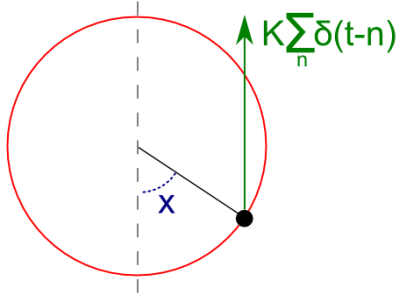
\includegraphics[width=0.33\textwidth]{kicked-rotor}

\begin{block}{Taylor, Chirikov and Greene  standard map}
\bea
x_{t+1} - x_{t} &=& p_{t+1} \qquad  \mod 1 \continue
p_{t+1} - p_{t} &=& F(x_{t})             \nnu
\eea
\end{block}

\medskip

\hfill $\to$ {\color{red}
chaos in Hamiltonian systems}
\end{frame} %%%%%%%%%%%%%%%%%%%%%%%%%%%%%%%%%%%%%%%%%%%%%%

\begin{frame}{the simplest example : a cat map evolving in time}

force
\(
 F(x) = Kx
\)
{\color{blue}linear} in the displacement $x$
\,,\;
$K\in\integers$
\bea
x_{t+1} &=& x_{t}+p_{t+1} \quad\;\;  \mod 1
        \continue
p_{t+1} &=& p_{t} + K x_{t} \qquad  \textcolor{red}{\mod 1}
\nnu
\eea
 \textcolor{red}{C}ontinuous
 \textcolor{red}{A}utomorphism of the
 \textcolor{red}{T}orus, or

\begin{block}{Hamiltonian cat map}
a linear, area preserving map of a 2-torus onto itself
 \[
 \left[\begin{array}{c}
   \ssp_{\zeit}  \\
   \ssp_{\zeit+1}
  \end{array} \right]=
  \jMps \left[\begin{array}{c}
   \ssp_{\zeit-1}  \\
   \ssp_{\zeit}
  \end{array} \right]
 - \left[\begin{array}{c}
 0  \\
 \Ssym{\zeit}
 \end{array} \right]
\,,\qquad
\jMps = \left[
\begin{array}{cc}
0 & 1 \\
-1 & s \\
\end{array}
    \right]
 \] %\ee{PerViv:2confRepMat}

\end{block}
for integer {\color{blue}`stretching' $s=\tr{\jMps} > 2$}
the map is \\ beloved by ergodicists :\\
hyperbolic $\Rightarrow$
{\color{blue}perfect chaotic Hamiltonian dynamical system}
\end{frame} %%%%%%%%%%%%%%%%%%%%%%%%%%%%%%%%%%%%%%%%%%%%%%

\begin{frame}{a cat is literally Hooke's wild, `anti-harmonic' sister}

\begin{block}{for $s<2$ Hooke rules}
local restoring oscillations

around the sleepy z-z-z-zzz resting state
\end{block}

\begin{block}{for $s>2$ cats rule}
exponential runaway

wrapped global around a \statesp\ torus
\end{block}
\bigskip

\hfill
{\color{red}cat} is to {\color{red}chaos}
what {\color{red}harmonic oscillator} is to {\color{red}order}
\vfill
\hfill
{\color{blue}there is no more fundamental example of chaos in mechanics}
\end{frame} %%%%%%%%%%%%%%%%%%%%%%%%%%%%%%%%%%%%%%%%%%%%%%

\begin{frame}{(2) a modern cat}
\vfill
\begin{center}
{\huge Lagrangian formulation}
\end{center}
\vfill
\end{frame} %%%%%%%%%%%%%%%%%%%%%%%%%%%%%%%%%%%%%%%%%%%%%%

\begin{frame}{cat map in Lagrangian form}
replace momentum by velocity
\[
p_{t+1}=(\ssp_{t+1}  - \ssp_{t})/\Delta t
\]
obtain
 \[
 \left[\begin{array}{c}
   \ssp_{\zeit}  \\
   \ssp_{\zeit+1}
  \end{array} \right]=
  \left[
\begin{array}{cc}
0 & 1 \\
-1 & s \\
\end{array}
    \right]
    \left[\begin{array}{c}
   \ssp_{\zeit-1}  \\
   \ssp_{\zeit}
  \end{array} \right]
 - \left[\begin{array}{c}
 0  \\
 \Ssym{\zeit}
 \end{array} \right]
 \] %\ee{PerViv:2confRepMat}

temporal lattice formulation % $(\ssp_{t},\ssp_{t-1})$
is {\Large pretty}\footfullcite{PerViv} :
\begin{block}{2-step difference equation}
\[
\ssp_{t+1}  -  s \, \ssp_{t} + \ssp_{t-1}
    =
-\Ssym{t}
\] %\ee{eq:CatMapNewton1}
\end{block}
integer $\Ssym{t}$ ensures that

\hfill $\ssp_{t}$ lands in the unit interval

\bigskip
\[
\Ssym{t}\in  \A
\,,\quad \A\ = \{\mbox{finite alphabet}\}
\]
\end{frame} %%%%%%%%%%%%%%%%%%%%%%%%%%%%%%%%%%%%%%%%%%%%%%

\begin{frame}{think globally, act locally}
\templatt\ at every instant $\zeit$, {\color{blue}local} in time
\[
\ssp_{t+1}  -  s \, \ssp_{t} + \ssp_{t-1}
    =
-\Ssym{t}
\] %\ee{eq:CatMapNewton1}
is enforced by the {\color{blue}global} equation
\beq
 \jMorb\,\Xx = -\Mm
\,,
\ee{catTempLatt}
where
\end{frame} %%%%%%%%%%%%%%%%%%%%%%%%%%%%%%%%%%%%%%%%%%%%%%

\begin{frame}{\jacobianOrb}
\[
 \jMorb\,\Xx + \Mm= 0
\]
with
\beq
{\Xx} % = \{\ssp_j\}
             = (\ssp_{\zeit+1},\cdots,\ssp_{\zeit+\cl{}})
\,,\quad
{\Mm} % = \{\Ssym{j}\}
             = (\Ssym{{\zeit+1}},\cdots,\Ssym{{\zeit+\cl{}}})
\ee{pathBern}
are a
{\color{blue}lattice state}, and a {\color{blue}symbol \brick}
\bigskip

and $[\cl{}\!\times\!\cl{}]$
 {\color{blue}\jacobianOrb} \jMorb\ is
\beq
\hopMat - s\id + \hopMat^{-1}
=  \left(\begin{array}{ccccc}
            -s    &  1    &        &   & 1\cr
             1    & -s    &   1    &   &  \cr
                  &  1    &        & \ddots &  \cr
                  &       &        &-s & 1 \cr
             1    &       &        &   &-s
          \end{array} \right)
\ee{hopMatrix}
\end{frame} %%%%%%%%%%%%%%%%%%%%%%%%%%%%%%%%%%%%%%%%%%%%%%

\begin{frame}{think globally, act locally}
solving the \templatt\ equation
\[
\jMorb\Xx= -\Mm
\,,
\]
with
the $[\cl{}\!\times\!\cl{}]$ matrix ~~~~~
\(
\jMorb = \hopMat - s\id + \hopMat^{-1}
\) %{tempBernFix}
\medskip

can be viewed as a search for zeros of the function
\beq
F[\Xx] = \jMorb\Xx+\Mm = 0
\ee{tempFixPoint}
where the entire {\color{blue}global lattice state} ${\Xx}_{\Mm}$ is
\medskip

a single {\color{blue}fixed point}
${\Xx}_{\Mm}=(\ssp_1,\ssp_{2},\cdots,\ssp_{\cl{}})$

\hfill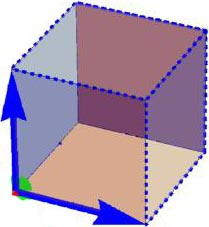
\includegraphics[width=0.12\textwidth]{hyperCube}

\hfill
in the \cl{}\dmn\ unit hyper-cube ~~~~~~~~~~~$\Xx\in[0,1)^\cl{}$
\end{frame} %%%%%%%%%%%%%%%%%%%%%%%%%%%%%%%%%%%%%%%%%%%%%%

\begin{frame}{fundamental fact in action}
% BernCyc2Jacob.svg
    \begin{block}{\templatt\  {\fundPip} for period 2}
square $[0BCD]$
$\Rightarrow\jMorb\,=\,$
{\fundPip} $[0B'C'D']$
\bigskip

\begin{center}
            \begin{minipage}[c]{0.32\textwidth}\begin{center}
% ChaosBook {fig:BernPartExam}
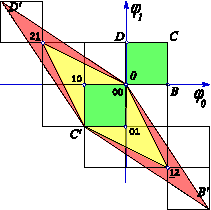
\includegraphics[width=1.0\textwidth]{catCyc2JacobUnit}
            \end{center}\end{minipage}
            \hspace{2ex}
            \begin{minipage}[c]{0.46\textwidth}
$N_2=|\Det\jMorb|=5$
\medskip

{\fundPip} \\
$=$  5 unit area quadrilaterals
            \end{minipage}
\end{center}
a periodic point per each unit volume
    \end{block}
\end{frame} %%%%%%%%%%%%%%%%%%%%%%%%%%%%%%%%%%%%%%%%%%%%%%

\begin{frame}{\templatt\  zeta function}
is the generating function that counts {\color{blue}orbits}
\medskip

substituting the {\color{blue}\HillDet} count of periodic lattice states
\[
N_n=|\Det\jMorb|
\]
into the
{topological} zeta func\-tion
\[
\zetatop(z)
  =   \exp \left(
    -\sum_{n=1} \frac{z^n}{n} N_n
    \right)
\]%\label{perOrbits:Isola90-13}
leads to the elegant explicit formula\footfullcite{Isola90}
\[
\zetatop(z)
 =  \frac{1 - s z + z^2}
         {1 - 2 z + z^2}
\]%\label{perOrbits:Isola90-13}


\vfill\hfill
{\Huge \textcolor{red}{solved!}}
\end{frame} %%%%%%%%%%%%%%%%%%%%%%%%%%%%%%%%%%%%%%%%%%%%%%

\begin{frame}{a side remark to experts}
% BernCyc2Jacob.svg
    \begin{block}{slicing cats}
\begin{center}
            \begin{minipage}[c]{0.23\textwidth}\begin{center}
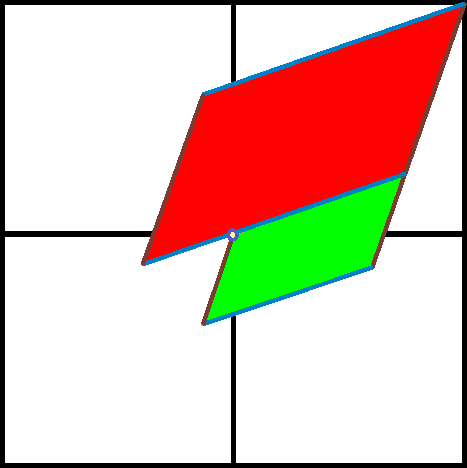
\includegraphics[width=1.0\textwidth]{PVAdlerWeissB-a}\\(a)
            \end{center}\end{minipage}
            \begin{minipage}[c]{0.23\textwidth}\begin{center}
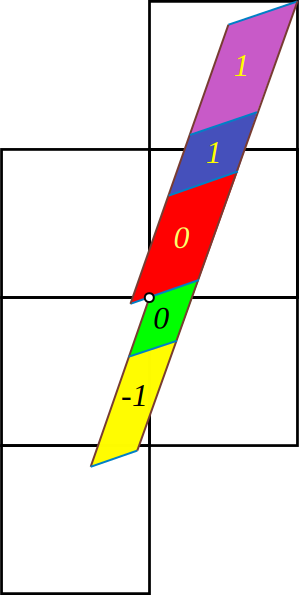
\includegraphics[width=1.0\textwidth]{PVAdlerWeissB-b}\\(b)
            \end{center}\end{minipage}
            \begin{minipage}[c]{0.23\textwidth}\begin{center}
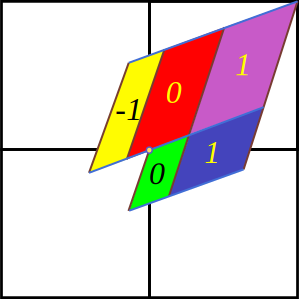
\includegraphics[width=1.0\textwidth]{PVAdlerWeissB-c}\\(c)
            \end{center}\end{minipage}
            ~~~
            \begin{minipage}[c]{0.12\textwidth}\begin{center}
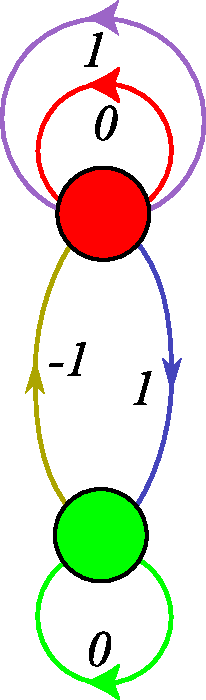
\includegraphics[width=1.0\textwidth]{PVAWMarkovCol}\\(d)
            \end{center}\end{minipage}
\end{center}

 is not the way
    \end{block}

\AW\ generating partition of the unit torus\\
is a distraction. Klein-Gordon is a deeper insight
\end{frame} %%%%%%%%%%%%%%%%%%%%%%%%%%%%%%%%%%%%%%%%%%%%%%

\begin{frame}{what continuum theory is \templatt\ discretization of?}
have
\begin{block}{2-step difference equation}
\[
\ssp_{t+1}  -  s \, \ssp_{t} + \ssp_{t-1}
    =
-\Ssym{t}
\] %\ee{eq:CatMapNewton1}
\end{block}
discrete lattice
\begin{block}{Laplacian in $1$ dimension}
\[
\ssp_{t+1} - 2\ssp_{t} + \ssp_{t-1}
     =
\Box\,\ssp_t
\]
\end{block}
\medskip

so \templatt\ is an (anti)oscillator chain, known as
\begin{block}{$d=1$ Klein-Gordon (or damped Poisson) equation (!)}
\[
 (-\Box + {\mu}^2)\,\ssp_{t} = \m_t
\,, \qquad
{\mu}^2= s-2
\] %\ee{LinearConn}
\end{block}
\vfill\hfill
\textcolor{red}{did you know that a cat map can be so cool?}
\end{frame} %%%%%%%%%%%%%%%%%%%%%%%%%%%%%%%%%%%%%%%%%%%%%%

\begin{frame}{a reminder slide, to skip : Helmholtz equation in continuum}
\begin{block}{inhomogeneous Helmoltz equation}
is an elliptical equation of form
\beq
   (\Box+k^2)\,\ssp(x)= -\Ssym{}(x)\,,\qquad x\in \reals^d
\label{CatMapContinuesPC}
\eeq
where $\ssp(x)$ is a $C^2$ function, and $\Ssym{}(x)$ is a function
with compact support
\end{block}

\bigskip

for the ${\mu}^2=-k^2>0$ (imaginary $k$), the equation is known as  the
{\color{blue}Klein-Gordon}, Yukawa, or
{\color{blue}screened Poisson equation}\footfullcite{FetWal03}
equation
\end{frame} %%%%%%%%%%%%%%%%%%%%%%%%%%%%%%%%%%%%%%%%%%%%%%

\begin{frame}{that's it! for spacetime of $1$ dimension}
lattice Klein-Gordon equation
    {\Huge
\[
  (-\Box + {\mu}^2)\,\ssp_{t} = \m_t
%    \,, \qquad
\] %\ee{LinearConn}
    }
\hfill solved completely and analytically!
\end{frame} %%%%%%%%%%%%%%%%%%%%%%%%%%%%%%%%%%%%%%%%%%%%%%


\begin{frame}{think globally, act locally - summary}
\bigskip
the problem of determining all global solutions stripped
to its bare essentials :
\bigskip
\begin{enumerate}
              \item
each solution a zero of the global {\color{blue}fixed point} condition
\[
F[\Xx] = 0
\]
              \item
compute  the {\jacobianOrb}
\[
\jMorb_{ij} =\frac{\delta F[\Xx]_i}{\delta \ssp_j}
\]
              \item
{\color{blue}fundamental fact} ~~~~~~~~
\(
N_\cl{} = |\Det\jMorb| =
\)
 period-$\cl{}$ states

 \bigskip
              \item
\hfill $\Rightarrow$ {\color{blue}zeta function} $\zetatop(z)$
            \end{enumerate}
\end{frame} %%%%%%%%%%%%%%%%%%%%%%%%%%%%%%%%%%%%%%%%%%%%%%

\section[\catlatt]
 {\catlatt}
\label{s:catLatt}

\begin{frame}{}
\begin{bartlett}{
Du mu{\ss}t es dreimal sagen!
        }
\bauthor{
Mephistopheles
    }
\end{bartlett}
\vfill
\begin{enumerate}
              \item \textcolor{gray}{\small
%what this is about
%              \item
coin toss
              \item
kicked rotor
                  }
              \item {\Large
\catlatt
                  }\textcolor{gray}{\small
              \item
bye bye, dynamics
                    }
            \end{enumerate}
\end{frame} %%%%%%%%%%%%%%%%%%%%%%%%%%%%%%%%%%%%%%%%%%%%%%

\begin{frame}{herding cats in $d$ spacetime dimensions}
start with
\begin{block}{a cat at each lattice site}
\bigskip

talk to neighbors
\medskip

spacetime $d$\dmn\
~~~~~~~ {\color{blue}\Large \catlatt}
\end{block}

\vfill

\begin{itemize}
  \item {\scriptsize Hamiltonian formulation is awkward, fuggedaboutit!}
  \item Lagrangian formulation is elegant
\end{itemize}
\end{frame} %%%%%%%%%%%%%%%%%%%%%%%%%%%%%%%%%%%%%%%%%%%%%%

\begin{frame}{spatiotemporally infinite `\catlatt'}
%\begin{center}
%\hfill
\includegraphics[width=0.55\textwidth]{spatiotempCat}
\hfill
\includegraphics[width=0.55\textwidth]{DawnBishopCats}
%\end{center}
\end{frame} %%%%%%%%%%%%%%%%%%%%%%%%%%%%%%%%%%%%%%%%%%%%%%

\begin{frame}{\catlatt}
consider
a 1 {\color{blue}spatial} dimension lattice, with field
$\ssp_{nt}$ \\
(the angle of a kicked
rotor ``particle'' at instant $t$, at site $n$)
\begin{block}{require}
\begin{itemize}
\item  each site couples to
its nearest neighbors $\ssp_{n\pm1,t}$
\item  invariance under
spatial translations
\item  invariance under spatial reflections
\item  invariance under the space-time exchange
\end{itemize}
\end{block}

\bigskip

Gutkin \& Osipov\footfullcite{GutOsi15} obtain
\begin{block}{2\dmn\ coupled cat map lattice}
\[
\ssp_{n,t+1} + \ssp_{n,t-1} - 2s \, \ssp_{n t} + \ssp_{n+1,t} + \ssp_{n-1, t}
     =-\Ssym{n t}
\] %\ee{eq:CatMapNewton2}
\end{block}
\end{frame} %%%%%%%%%%%%%%%%%%%%%%%%%%%%%%%%%%%%%%%%%%%%%%

\begin{frame}{\catlatt\ : a strong coupling field theory}
symmetries : translations $\circ$ time-reversal $\circ$ spatial reflections

\bigskip

\begin{block}{the key assumption}
\begin{itemize}
\item  invariance under the space-time exchange
\end{itemize}
\end{block}
\bigskip

{\color{red}not} a traditional \\
{\color{blue}spatially
weakly coupled} lattice model\footfullcite{BunSin88}
\bigskip
%assuming that coupling strengths along the time and space directions are
%the same makes \catlatt\ a maximally strongly coupled field theory
%
%
%
%in contrast to the usual weak-coupling lattice models
\vfill

\begin{itemize}
  \item \catlatt\ is a Euclidean field theory
%  \item in Lagrangian formulation
\end{itemize}
\end{frame} %%%%%%%%%%%%%%%%%%%%%%%%%%%%%%%%%%%%%%%%%%%%%%

\begin{frame}{herding cats : a discrete Euclidean space-time field theory}
write the spatial-temporal differences as discrete derivatives
\begin{block}{Laplacian in %$d=1$ and
              $d=2$ dimensions}
%\(
%\Box\,\ssp_t \;\;\,=\, \ssp_{t+1} - 2\ssp_{t} + \ssp_{t-1}
%\)\\
\(
\Box\,\ssp_{nt} \,=\, \ssp_{n,t+1} + \ssp_{n,t-1}
- 4 \, \ssp_{nt} + \ssp_{n+1,t} + \ssp_{n-1, t}
\)\\
~~~~{\scriptsize subtract 2\dmn\ coupled cat map lattice equation}\\
\(
-\Ssym{n t}
 =
\ssp_{n,t+1} + \ssp_{n,t-1} - 2s \, \ssp_{n t} + \ssp_{n+1,t} + \ssp_{n-1, t}
\) %\ee{eq:CatMapNewton2}
\end{block}

\bigskip

{\color{blue}cat herd} is thus governed by the law of
\begin{block}{$d$\dmn\ \catlatt}
\[
 (-\Box + {\mu}^2)\,\ssp_{z} = \m_z
\,, \qquad
{\mu}^2= d(s-2)
\] %\ee{LinearConn}

\medskip

\end{block}

\bigskip

where
\(
  \ssp_{z} \in [0,1)
    \,, \quad
  \Ssym{z} \in \A
    \mbox{  and  }
  z\in \integers^{d}
\) = integer lattice
\end{frame} %%%%%%%%%%%%%%%%%%%%%%%%%%%%%%%%%%%%%%%%%%%%%%

\begin{frame}{discretized linear PDE}
\begin{block}{$d$\dmn\ \catlatt}
{\Large
\[
 (-\Box + {\mu}^2)\,\ssp_{z} = \m_z
\] %\ee{LinearConn}
}
\end{block}

\bigskip

is linear and known as
\begin{itemize}
\item {\color{blue}tight-binding} model or {\color{blue}Helmholtz} equation \\
if stretching is weak, $s<2$ \\
 $[$oscillatory sine, cosine solutions]
\item
Euclidean {\color{blue}Klein-Gordon} or (damped {\color{blue}Poisson})\\
if stretching is strong, $s>2$ \\
 $[$hyperbolic sinches, coshes, `{\color{blue}mass}' ${\mu}^2=d(s-2)$]
\end{itemize}
\medskip

nonlinearity is hidden in the `sources'
\[
  \Ssym{z} \in \A
    \mbox{  at lattice site  }
  z\in \integers^{d}
\]
\end{frame} %%%%%%%%%%%%%%%%%%%%%%%%%%%%%%%%%%%%%%%%%%%%%%

\begin{frame}{spring mattress vs field of rotors}
\begin{center}
            \begin{minipage}[c]{0.40\textwidth}\begin{center}
traditional field theory
\bigskip

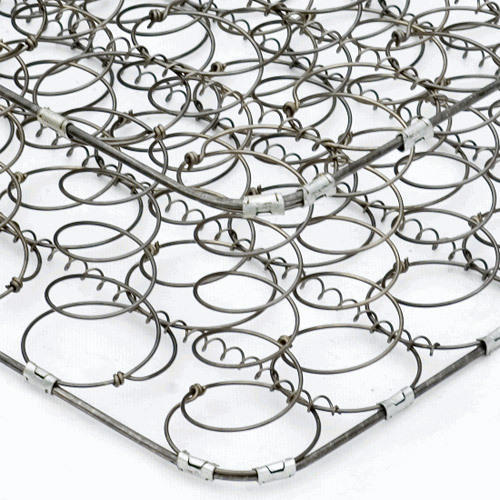
\includegraphics[width=0.85\textwidth]{mattressSpring}\\
{\color{blue}Helmholtz}
            \end{center}\end{minipage}
            \hspace{2ex}
            \begin{minipage}[c]{0.46\textwidth}\begin{center}
chaotic field theory\\
\bigskip
\bigskip
\bigskip

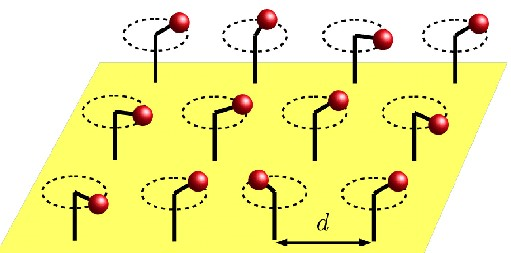
\includegraphics[width=1.0\textwidth]{flagellum1}\\
\bigskip

damped {\color{blue}Poisson}
            \end{center}\end{minipage}
\end{center}
\end{frame} %%%%%%%%%%%%%%%%%%%%%%%%%%%%%%%%%%%%%%%%%%%%%%

\begin{frame}{the simplest of all `turbulent' field theories ! }
\catlatt
\[
 (-\Box + {\mu}^2)\,\ssp_{z} = \m_z
\] %\ee{LinearConn}
\bigskip
\hfill can be solved completely (?) and analytically (!)

\bigskip
\bigskip

assign to each site $z$ a
letter \Ssym{z}\ from the alphabet $\A$.

\medskip

a particular fixed set
of letters  \Ssym{z}\ (a symbol \brick)
\[
\Mm= \{\Ssym{z}\} % \in \A \,,\; z\in \integers^d \}
 = \{\Ssym{n_1 n_2 \cdots n_d}\}
\,,
\]
is a complete specification of  \\
the corresponding lattice state $\Xx$
\bigskip

{\color{blue}\footnotesize
from now on work in $d=2$ dimensions, `stretching parameter'
$s=5/2$
}
\end{frame} %%%%%%%%%%%%%%%%%%%%%%%%%%%%%%%%%%%%%%%%%%%%%%

\begin{frame}{think globally, act locally}
solving the \catlatt\ equation
\[
\jMorb\Xx= -\Mm
\,,
\]
with
the $[\cl{}\!\times\!\cl{}]$ matrix ~~~~~
\(
\jMorb = \sum_{j=1}^{2}\left(\hopMat_j-{s}\unit+\hopMat_{j}^{-1}\right)
\) %{tempBernFix}
\medskip

can be viewed as a search for zeros of the function
\beq
F[\Xx] = \jMorb\Xx+\Mm = 0
\ee{tempFixPoint}
where the entire {\color{blue}global lattice state} ${\Xx}_{\Mm}$ is
\medskip

a single {\color{blue}fixed point}
${\Xx}_{\Mm}=\{\ssp_z\}$

\hfill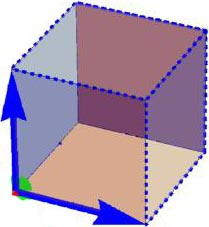
\includegraphics[width=0.12\textwidth]{hyperCube}

\hfill
in the \speriod{}\period{}\dmn\ unit hyper-cube $\Xx\in[0,1)^{\speriod{}\period{}}$
\medskip

$\speriod{}$ is the `spatial',
$\period{}$ the `temporal' lattice period
\end{frame} %%%%%%%%%%%%%%%%%%%%%%%%%%%%%%%%%%%%%%%%%%%%%%

\begin{frame}{think globally, act locally}
    \begin{center}
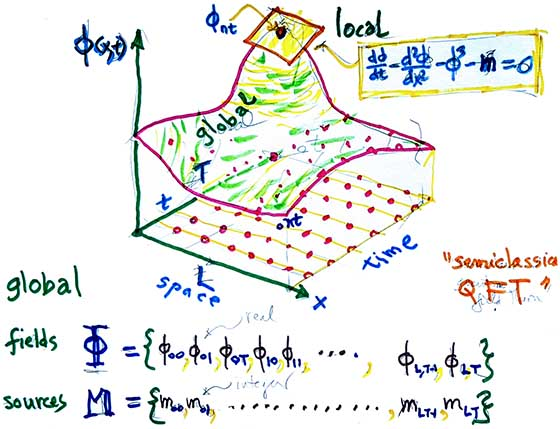
\includegraphics[width=0.85\textwidth]{globalLocal}
    \end{center}
for each symbol array \Mm, a periodic lattice state $\Xx_\Mm$
\end{frame} %%%%%%%%%%%%%%%%%%%%%%%%%%%%%%%%%%%%%%%%%%%%%%

\begin{frame}{next, enumerate all periodic spacetime tilings of the  integer lattice}
each tile : 2\dmn\ {(sub)lattice}, an infinite array of points
\beq
\Lambda = \{n_1 {\bf a}_1 + n_2 {\bf a}_2\,|\,n_i \in \mathbb{Z}\}
\ee{2DBravaisLattice}
with the defining tile spanned by a pair of basis vectors
$\mathbf{a}_{1},\mathbf{a}_{2}$

    \begin{block}{example : four tiles of area 10}
\hfill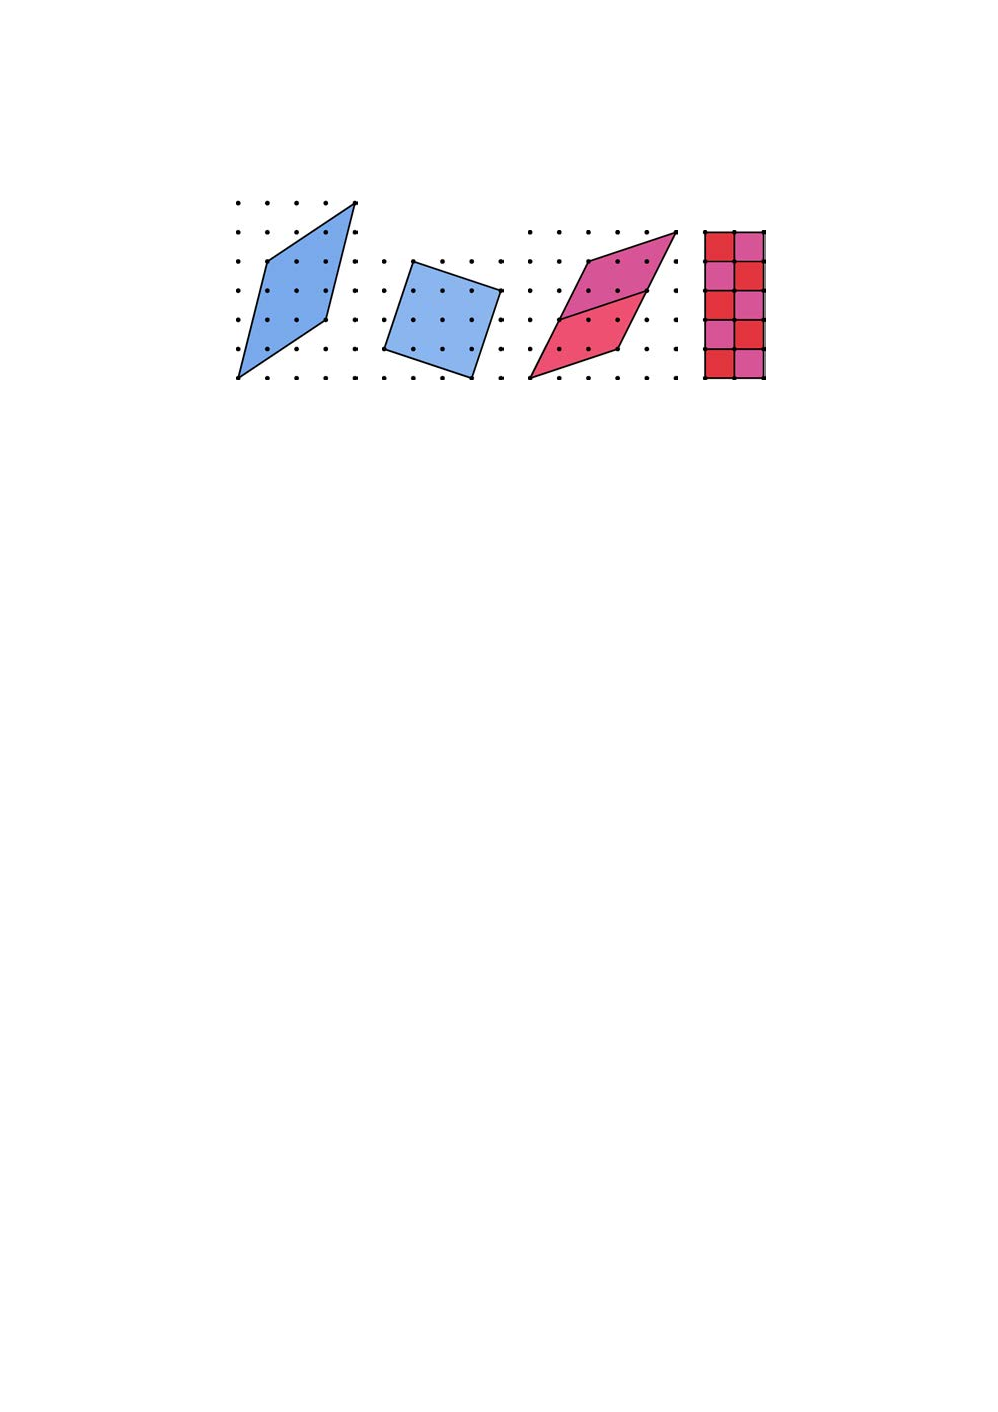
\includegraphics[width=0.7\textwidth]{Holmin15-Fig1}
    \end{block}
\bigskip
The two blue tiles appear
`prime', \ie, not
tiled by smaller tiles.
\textcolor{red}{False!}~~~~~
all four big tiles can tilled by smaller ones.
%          }\label{Holmin15-Fig1}

\vfill\hfill
{\Huge \textcolor{red}{tricky!}}
\end{frame} %%%%%%%%%%%%%%%%%%%%%%%%%%%%%%%%%%%%%%%%%%%%%%

\begin{frame}{$2$\dmn\ lattice tilings}
2\dmn\ {\color{blue}\emph{lattice}} is
defined by a $[2\times2]$ {\color{blue}\fundPip} matrix whose columns are basis vectors
\[
\mathbf{A} =
\left[ \mathbf{a}_{1} \mathbf{a}_{2} \right]
 =
\left[
\begin{array}{cc}
\speriod{} & \tilt{} \\
0 & \period{}
\end{array}
\right]
\,,
\]
$\speriod{}$, $\period{}$ : spatial, temporal
lattice periods\\
`tilt'  $0\leq\tilt{}<\speriod{}$ imposes the
{\color{blue}\emph{relative-periodic}}\\
(\emph{`helical'}, \emph{`toroidal'},
\emph{`twisted'}, \emph{`screw'},  $\cdots$
) {\bcs}

    \begin{block}{example : $[3\!\times\!2]_1$ tile}
\begin{center}
            \begin{minipage}[c]{0.32\textwidth}\begin{center}
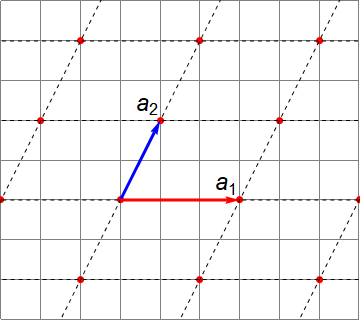
\includegraphics[width=1.0\textwidth]{HLBravaisLattice}
            \end{center}\end{minipage}
            \hspace{2ex}
            \begin{minipage}[c]{0.46\textwidth}
basis vectors
\\

${\bf a}_1=\left(
 \begin{array}{c}
 3\\
 0
 \end{array}
 \right)$,
${\bf a}_2=\left(
 \begin{array}{c}
 1\\
 2
 \end{array}
 \right)$
            \end{minipage}


\end{center}
    \end{block}
\end{frame} %%%%%%%%%%%%%%%%%%%%%%%%%%%%%%%%%%%%%%%%%%%%%%

\begin{frame}{exponentially many periodic lattice states in Felinestan}
\begin{center}
%%%%%%%%%%%%%%%%%%%%%%%%%%%%%%%%%%%%%%%%%%%%%%%%%%%%%%%%%%%%%
% HL 2020-06-09 siminos/figSrc/han/Mathematica/ColorBlock.nb
%\begin{figure}\begin{center}
            \begin{minipage}[c]{0.25\textwidth}\begin{center}
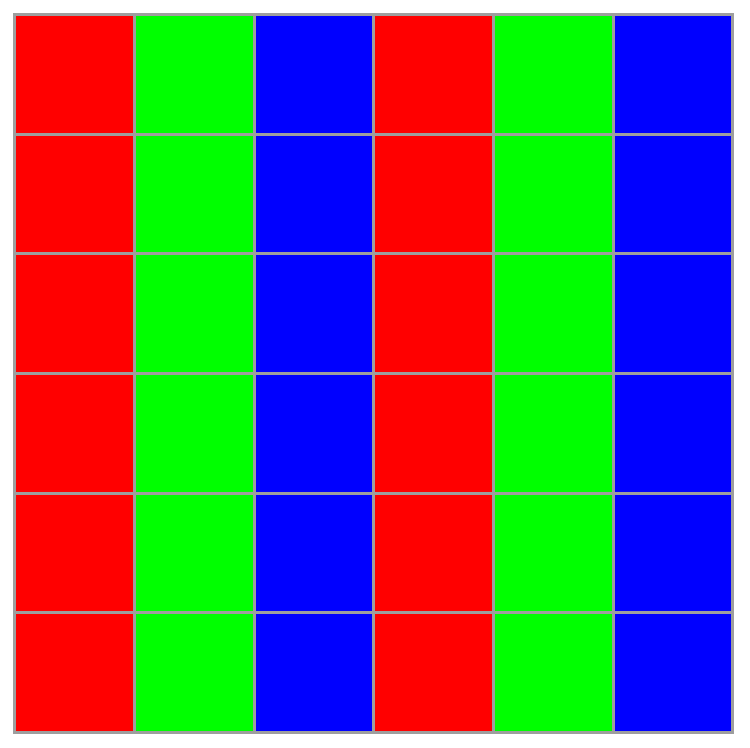
\includegraphics[width=1.0\textwidth]{HL310Block}\\$\BravCell{3}{1}{0}$ %(a)
            \end{center}\end{minipage}
            \hskip 4ex
            \begin{minipage}[c]{0.25\textwidth}\begin{center}
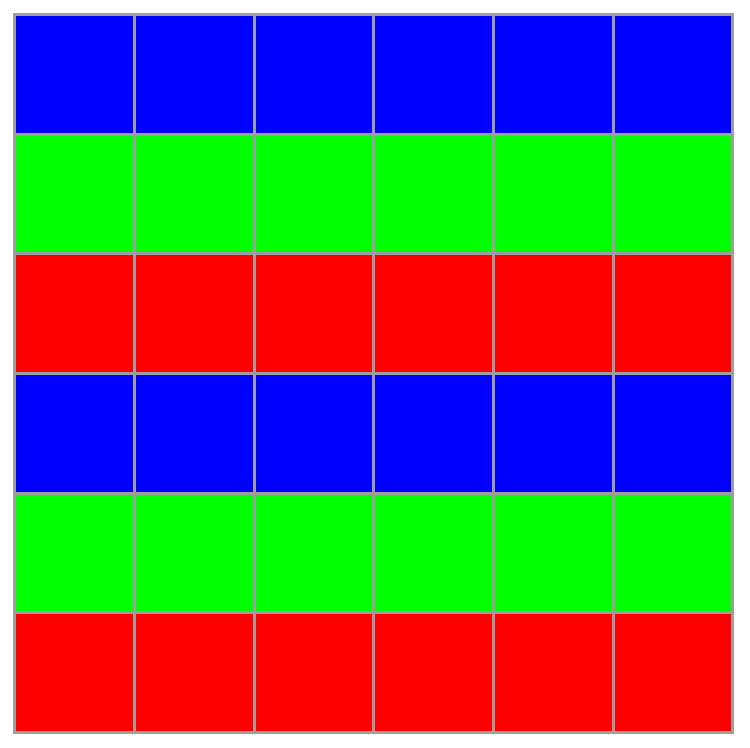
\includegraphics[width=1.0\textwidth]{HL130Block}\\$\BravCell{1}{3}{0}$ %(b)
            \end{center}\end{minipage}
            \hskip 4ex
            \begin{minipage}[c]{0.25\textwidth}\begin{center}
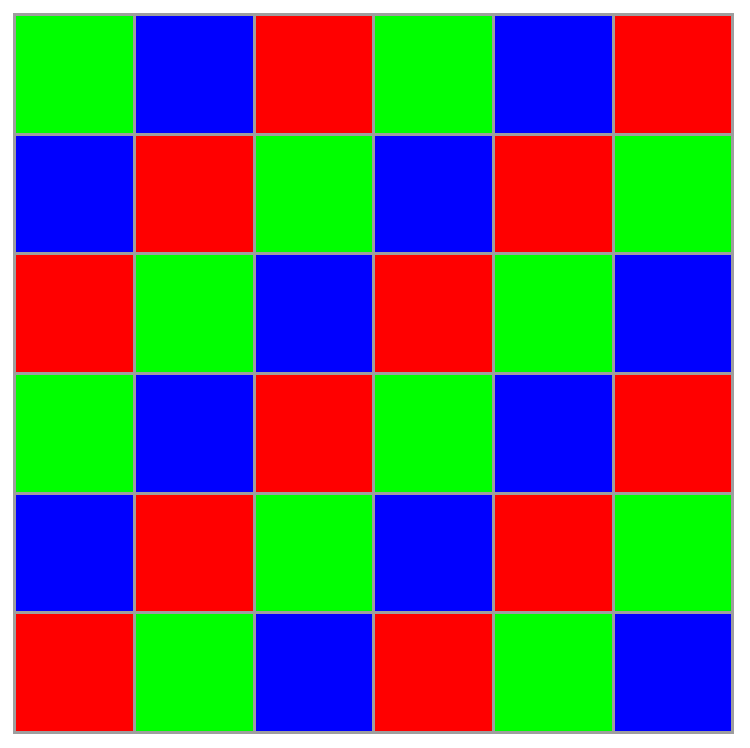
\includegraphics[width=1.0\textwidth]{HL311Block}\\$\BravCell{3}{1}{1}$ %(c)
            \end{center}\end{minipage}
%\end{center}
%  \caption{\label{fig:SpecialBravaisLatt}
%Examples of $\LTS{}{}{}$ periodic \brick s
%together with their \spt\ Bravais lattice tilings \refeq{2DBravaisLattice}.
%(a)
%$\BravCell{3}{1}{0}$, basis vectors
%$\mathbf{a}_1=\{3,0\}$ and $\mathbf{a}_2=\{0,1\}$;
%(b)
%$\BravCell{1}{3}{0}$, basis vectors
%$\mathbf{a}_1=\{1,0\}$ and $\mathbf{a}_2=\{0,3\}$;
%(c)
%$\BravCell{3}{1}{1}$, basis vectors
%$\mathbf{a}_1=\{3,0\}$ and $\mathbf{a}_2=\{1,1\}$;
%}
%%%%%%%%%%%%%%%%%%%%%%%%%%%%%%%%%%%%%%%%%%%%%%%%%%%%%%%%%%%%%
% HL 2020-06-09 siminos/figSrc/han/Mathematica/ColorBlock.nb
%\begin{figure}\begin{center}
            \begin{minipage}[c]{0.25\textwidth}\begin{center}
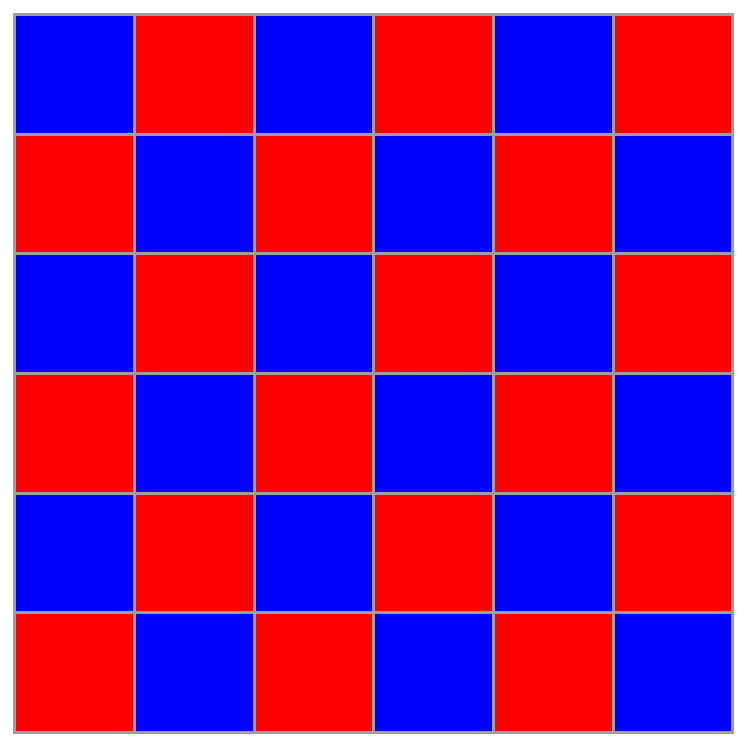
\includegraphics[width=1.0\textwidth]{HL211Block}\\$\BravCell{2}{1}{1}$ %(a)
            \end{center}\end{minipage}
            \hskip 4ex
            \begin{minipage}[c]{0.25\textwidth}\begin{center}
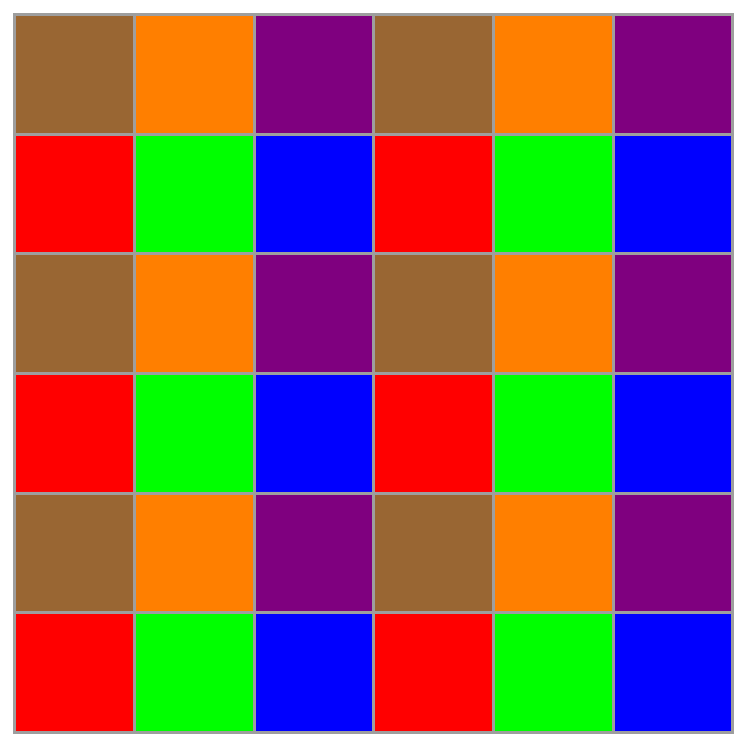
\includegraphics[width=1.0\textwidth]{HL320Block}\\$\BravCell{3}{2}{0}$ %(b)
            \end{center}\end{minipage}
            \hskip 4ex
            \begin{minipage}[c]{0.25\textwidth}\begin{center}
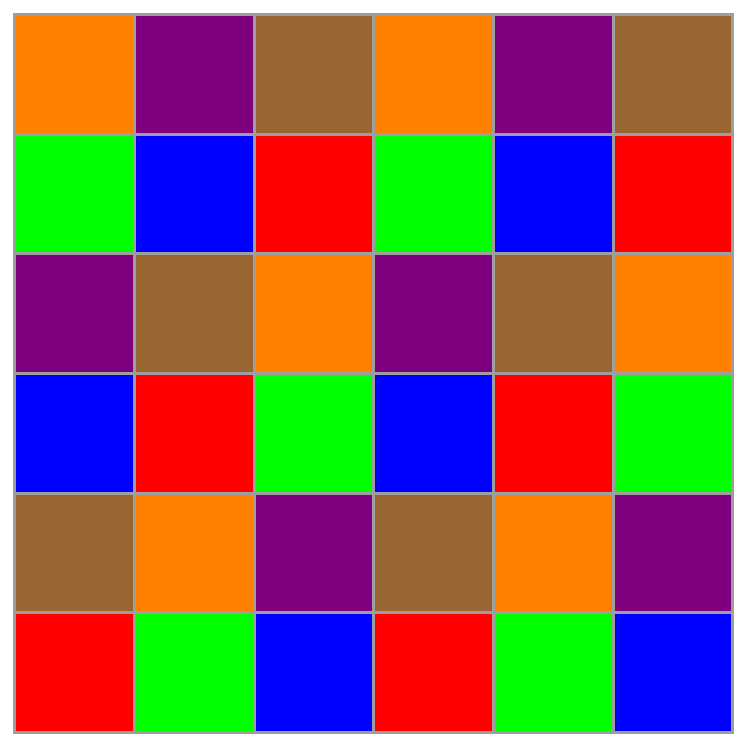
\includegraphics[width=1.0\textwidth]{HL321Block}\\$\BravCell{3}{2}{1}$ %(c)
            \end{center}\end{minipage}
%\end{center}
%  \caption{\label{fig:3x2rpo}
%Examples of $\LTS{}{}{}$ periodic \brick s
%together with their \spt\ Bravais lattice tilings \refeq{2DBravaisLattice}.
%(a)
%$\BravCell{2}{1}{1}$, basis vectors
%$\mathbf{a}_1=\{2,0\}$ and $\mathbf{a}_2=\{1,1\}$;
%(b)
%$\BravCell{3}{2}{0}$, basis vectors
%$\mathbf{a}_1=\{3,0\}$ and $\mathbf{a}_2=\{0,2\}$;
%(c)
%$\BravCell{3}{2}{1}$, basis vectors
%$\mathbf{a}_1=\{3,0\}$ and $\mathbf{a}_2=\{1,2\}$;
%}
%%%%%%%%%%%%%%%%%%%%%%%%%%%%%%%%%%%%%%%%%%%%%%%%%%%%%%%%%%%%%%%
\end{center}
tile {\color{green}color} = value of symbol $\Ssym{z}$
\end{frame} %%%%%%%%%%%%%%%%%%%%%%%%%%%%%%%%%%%%%%%%%%%%%%

%\begin{frame}{lattices, sublattices}
%2\dmn\ \emph{lattice} is an infinite array of points
%\beq
%\Lambda = \{n_1 {\bf a}_1 + n_2 {\bf a}_2\,|\,n_i \in \mathbb{Z}\}
%\ee{2DBravaisLattice}
%    \begin{block}{example : $[3\!\times\!2]_1$ tile}
%\begin{center}
%            \begin{minipage}[c]{0.32\textwidth}\begin{center}
%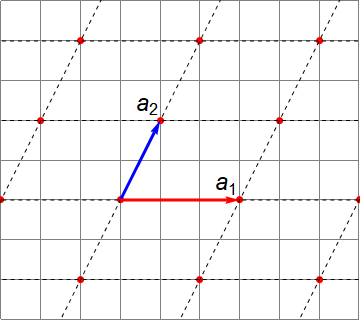
\includegraphics[width=1.0\textwidth]{HLBravaisLattice}
%            \end{center}\end{minipage}
%            \hspace{2ex}
%            \begin{minipage}[c]{0.46\textwidth}
%basis vectors \\ ${\bf a}_1=(3,0)$, ${\bf a}_2=(1,2)$
%            \end{minipage}
%\end{center}
%    \end{block}
%
%\vfill
%
%6 field values, on 6 lattice sites $z=(n,\zeit)$,
%$[3\!\times\!2]$ rectangle:
%\[
% \left[
% \begin{array}{ccc}
% \ssp_{01} & \ssp_{11} & \ssp_{21} \\
% \ssp_{00} & \ssp_{10} & \ssp_{20}
% \end{array}
% \right]
%\]
%\end{frame} %%%%%%%%%%%%%%%%%%%%%%%%%%%%%%%%%%%%%%%%%%%%%%
%

\begin{frame}{note : \catlatt\ dances over a parquet floor}
\begin{itemize}
  \item[(so far)]
latticization of spacetime continuum :\\
{\color{blue}\emph{field}} $\ssp(x,\zeit)$ over spacetime coordinates
$(x,\zeit)$\\ for {\color{blue}\emph{any}} field theory

~~~~~~~~~~~~~~~$\Rightarrow$

set of lattice site values $\ssp_z=\ssp(n\Delta{L},\zeit\Delta{T})$.\\
Subscript $z=(n,\zeit)\in\integers^d$ is a discrete $d$\dmn\
spacetime {\color{blue}\emph{coordinate}} over which the field $\ssp$ lives
\medskip

distinct spacetime tiles have tilted shapes
$\LTS{}{}{}$
\bigskip

  \item[(next)]
\catlatt\ {\color{blue}\emph{field}} $\ssp_{z}$ is confined to $[0,1)$\\
That imparts a $\integers^1$ lattice structure on {\fundPip} $\jMorb$
basis vectors ; fundamental fact then counts all periodic
{\color{blue}lattice \emph{states}} $\Xx_\Mm$ for \\
a given spacetime tile
$\LTS{}{}{}$
\end{itemize}
\end{frame} %%%%%%%%%%%%%%%%%%%%%%%%%%%%%%%%%%%%%%%%%%%%%%


\begin{frame}{fundamental fact works for a spacetime lattice (!)}

    \begin{block}{recall Bernoulli fundamental fact example ?}
\begin{center}
            \begin{minipage}[c]{0.32\textwidth}\begin{center}
% ChaosBook {fig:BernPartExam} % BernCyc2Jacob.svg
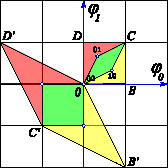
\includegraphics[width=1.0\textwidth]{BernCyc2JacobUnit}
            \end{center}\end{minipage}
            \hspace{2ex}
            \begin{minipage}[c]{0.46\textwidth}
unit hyper-cube $\Xx\in[0,1)^2$
\medskip

~~~~~~~~~~~~~~~~$\Rightarrow\jMorb\Rightarrow$
\medskip

{\fundPip}
            \end{minipage}
\end{center}
%$\jMorb\,[0BCD] =$ {\fundPip} $[0B'C'D']$
    \end{block}

\vfill

spacetime {\fundPip} basis
vectors $\jEigvec[j]$ \\
$=$ columns of the {\color{blue}\jacobianOrb}
\beq
\jMorb = (\jEigvec[1]|\jEigvec[2]|\cdots|\jEigvec[\speriod{}\period{}])
\ee{lattJac}
\end{frame} %%%%%%%%%%%%%%%%%%%%%%%%%%%%%%%%%%%%%%%%%%%%%%


%\begin{frame}{solving $1D$ cat map using Green's functions}
%\begin{block}{the Green's function $\Xx=g\,\Mm$ for a period \period{} solution of}
%\[
% (\Box -s+2)\ssp_{t} = \m_t
%%    \,, \qquad
%\] %\ee{LinearConn}
%
%\medskip
%\end{block}
%\begin{block}{is a Toeplitz matrix $\gd$ that satisfies}
%\bea
% (\D \gd)_{tt'}&=&\delta_{tt'}\,, \qquad t,t'\in 0,1,2,\cdots,\period{}-1
%% \label{1DGreenFun0} \ee{1DGreenFunDirichlet}
%        \continue
%   & &  \continue
%\D &=&\left(\begin{array}{ccccccc}
% s&-1 & 0 & 0 &\dots &0&-1 \\
%-1 &  s&-1 & 0 &\dots &0&0 \\
%0 &-1 &  s&-1 &\dots &0 & 0 \\
%\vdots & \vdots &\vdots & \vdots & \ddots &\vdots &\vdots\\
%0 & 0 & \dots &\dots &\dots  & s&-1 \\
%-1 & 0 & \dots &  \dots &\dots&-1 &  s
%        \end{array} \right )
%\nnu
%\eea %ee{3diagToeplitz}
%\medskip
%\end{block}
%\end{frame} %%%%%%%%%%%%%%%%%%%%%%%%%%%%%%%%%%%%%%%%%%%%%%

%\begin{frame}{
%the 3-letter translations alphabet \;+\; the Markov graph
%             }
%
%\medskip
%
%generates the admissible orbits of $1D$ cat map
%\[ %beq
%\Ssym{t}\in\{\underline{1},0,1\}
%\] %ee{threeLett}
%example : all admissible 4-cycles
%\bea
%{\bf x}_{0 0 1 \underline{1}} &=& \frac{1}{15}
%\left[
%\begin{array}{cccc}
% {-1} &
% {1} &
% {4} &
% {-4}
%\end{array}
%\right]
%    \,,\qquad
%{\bf x}_{0 1 0 \underline{1}}= \frac{1}{15}
%\left[
%\begin{array}{cccc}
% {0} &
% {5} &
% {0} &
% {-5}
%\end{array}
%\right]
%    \continue
%{\bf x}_{0 1 \underline{1}1} &=& \frac{1}{15}
%\left[
%\begin{array}{cccc}
% {4} &
% {6} &
% {-1} &
% {6}
%\end{array}
%\right]
%    \,,\qquad
%{\bf x}_{0 1 1 \underline{1}}= \frac{1}{15}
%\left[
%\begin{array}{cccc}
% {2} &
% {8} &
% {7} &
% {-2}
%\end{array}
%\right]
%    \continue
%% Predrag 2018-02-19 replaced the
%% old 6 \cycle{3125} \\  1 0 1 \underline{1} = 4 \cycle{1253}
%% by new No. 6:
%% 6 \cycle{1133} \\  0 0 1            1
%{\bf x}_{0 0 1 1} &=& \frac{1}{15}
%\left[
%\begin{array}{cccc}
% {5} &
% {5} &
% {10} &
% {10}
%\end{array}
%\right]
%    \,,\qquad
%{\bf x}_{1 1 1 \underline{1}}= \frac{1}{15}
%\left[
%\begin{array}{cccc}
% {9} &
% {11} &
% {9} &
% {1}
%\end{array}
%\right]
%    \continue
%{\bf x}_{1 1 1 0} &=& \frac{1}{15}
%\left[
%\begin{array}{cccc}
% {12} &
% {13} &
% {12} &
% {8}
%\end{array}
%\right]
%    \,,\qquad
%{\bf x}_{1 1 0 \underline{1}}= \frac{1}{15}
%\left[
%\begin{array}{cccc}
% {7} &
% {8} &
% {2} &
% {-2}
%\end{array}
%\right]
%    \continue
%{\bf x}_{0 0 \underline{1}1} &=& \frac{1}{15}
%\left[
%\begin{array}{cccc}
% {1} &
% {-1} &
% {-4} &
% {4}
%\end{array}
%\right]
%\label{4cyclesPerPoints}
%\eea
%\end{frame} %%%%%%%%%%%%%%%%%%%%%%%%%%%%%%%%%%%%%%%%%%%%%%

\begin{frame}{example : spacetime periodic $\BravCell{3}{2}{0}$
              lattice state}
\[
F[\Xx] = \jMorb\Xx+\Mm = 0
\]
6 field values, on 6 lattice sites $z=(n,\zeit)$,
$\BravCell{3}{2}{0}$ tile :
\[
\Xx_{\BravCell{3}{2}{0}} =
 \left[
 \begin{array}{ccc}
 \ssp_{01} & \ssp_{11} & \ssp_{21} \\
 \ssp_{00} & \ssp_{10} & \ssp_{20}
 \end{array}
 \right]
\,,\qquad %\Leftrightarrow\qquad
6\,\Mm_{\BravCell{3}{2}{0}} =
%%%%%%%%%%%%%%%%%%%%%%%%%%%%%%%%%%%%%%%%%%%%%%%%%%%%%%%%%%%%%
% HL 2020-06-09 siminos/figSrc/han/Mathematica/ColorBlock.nb
            \begin{minipage}[c]{0.15\textwidth}\begin{center}
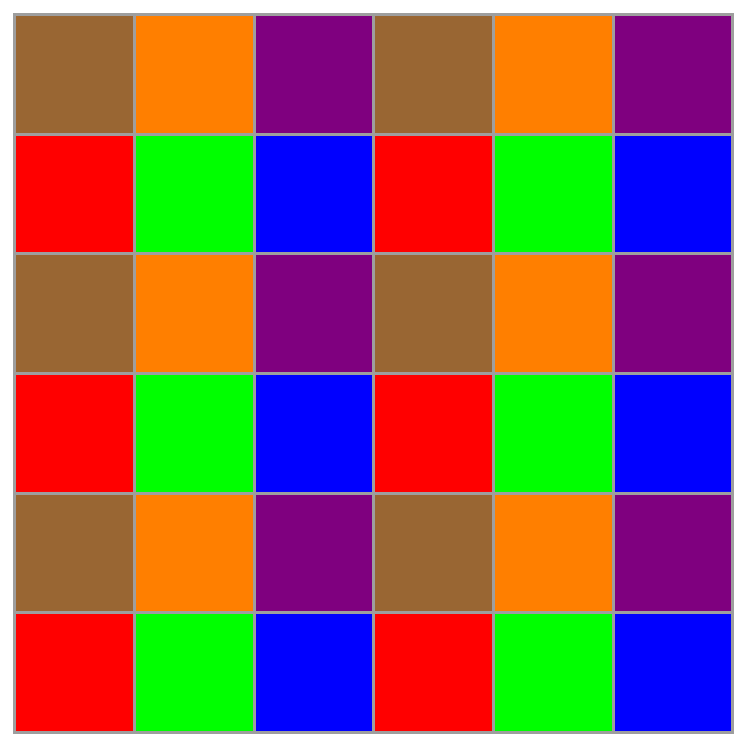
\includegraphics[width=1.0\textwidth]{HL320Block} %\\$\BravCell{3}{2}{0}$ %(b)
            \end{center}\end{minipage}
\]
where the region of symbol plane shown is tiled by 6 repeats of the
$\Mm_{\BravCell{3}{2}{0}}$ \brick, and tile {\color{green}color} = value of
symbol $\Ssym{z}$
\medskip

`stack up' vectors and matrices, vectors as 1\dmn\ arrays,
\beq
\Xx_{\BravCell{3}{2}{0}} =
\left(\begin{array}{c}
 \ssp_{01} \\
 \ssp_{00} \\
  \hline
 \ssp_{11} \\
 \ssp_{10} \\
  \hline
 \ssp_{21} \\
 \ssp_{20} \\
      \end{array}\right)
\,,\qquad
\Mm_{\BravCell{3}{2}{0}} =
\left(\begin{array}{c}
 \Ssym{01} \\
 \Ssym{00} \\
  \hline
 \Ssym{11} \\
 \Ssym{10} \\
  \hline
 \Ssym{21} \\
 \Ssym{20} \\
        \end{array}\right)
\ee{3times2blockVect}
\end{frame} %%%%%%%%%%%%%%%%%%%%%%%%%%%%%%%%%%%%%%%%%%%%%%

\begin{frame}{}
with the $[6\!\times\!6]$ {\jacobianOrb} in block-matrix form
\beq
\jMorb_{\BravCell{3}{2}{0}} =
\left(
\begin{array}{cc|cc|cc}
 -2 s & 2 & 1 & 0 & 1 & 0  \\
 2 & -2 s & 0 & 1 & 0 & 1  \\
  \hline
 1 & 0 & -2 s & 2 & 1 & 0  \\
 0 & 1 & 2 & -2 s & 0 & 1  \\
  \hline
 1 & 0 & 1 & 0 & -2 s & 2  \\
 0 & 1 & 0 & 1 & 2 & -2 s
\end{array}
\right)
\ee{3times2basisVecs}
\end{frame} %%%%%%%%%%%%%%%%%%%%%%%%%%%%%%%%%%%%%%%%%%%%%%

\begin{frame}{}

{\fundPip} basis
vectors $\jEigvec[j]$ are
the columns of the {\jacobianOrb}
\beq
\jMorb_{\BravCell{3}{2}{0}} =
\left(
\begin{array}{c|c|c|c|c|c}
 -2 s & 2 & 1 & 0 & 1 & 0  \\
 2 & -2 s & 0 & 1 & 0 & 1  \\
 1 & 0 & -2 s & 2 & 1 & 0  \\
 0 & 1 & 2 & -2 s & 0 & 1  \\
 1 & 0 & 1 & 0 & -2 s & 2  \\
 0 & 1 & 0 & 1 & 2 & -2 s
\end{array}
\right)
\ee{3times2basisVecs}
the `fundamental fact' now yields the number of
solutions for any half-integer ${s}$ as {\color{blue}\HillDet}
\beq
N_{\BravCell{3}{2}{0}} = |\Det\jMorb_{\BravCell{3}{2}{0}}|
                   = 4({s}-2)s(2{s}-1)^2 (2{s}+3)^2
\ee{N3times2}
\end{frame} %%%%%%%%%%%%%%%%%%%%%%%%%%%%%%%%%%%%%%%%%%%%%%

\begin{frame}{can count \catlatt\ states for any $\Lambda=\LTS{}{}{}$}
\begin{center}
{\scriptsize
\begin{tabular}{lllr}
\\[-16pt]
$~~~\Lambda$
                         & ~~~$N_\Lambda(s)$ & $M_\Lambda(s)$
                                                 &$R$  \\
\hline
$\BravCell{1}{1}{0}$    &   $2({s}-2)$ & $2({s}-2)$ & 1 \\
$\BravCell{2}{1}{0}$    &   $2({s}-2)2s$ & $2({s}-2)\frac{1}{2}(2{s}-1)$   & 2 \\
$\BravCell{2}{1}{1}$  &   $2({s}-2)2({s}+2)$ & $2({s}-2)\frac{1}{2}(2{s}+3)$  & \\
$\BravCell{3}{1}{0}$    &   $2({s}-2)(2{s}-1)^2$ & $2({s}-2)\frac{4}{3}({s}-1){s}$ &  \\
$\BravCell{3}{1}{1}$  &   $2({s}-2)4({s}+1)^2$ & $2({s}-2)\frac{1}{3}(2{s}+1)(2{s}+3)$ & \\
%was $2({s}-2)(2{s}-1)^2$
%$\BravCell{3}{1}{2}$  &   $2({s}-2)4({s}+1)^2$ & $2({s}-2)\frac{1}{3}(2{s}+1)(2{s}+3)$ & \\
%was $2({s}-2)(2{s}-1)^2$
$\BravCell{4}{1}{0}$    &   $2({s}-2)8({s}-1)^2{s}$ & $2({s}-2)\frac{1}{2}(2{s}-3)(2{s}-1)s$ & \\
$\BravCell{4}{1}{1}$  &   $2({s}-2)8s^2({s}+2)$ & $2({s}-2)\frac{1}{2}({s}+2)(2{s}-1)(2{s}+1)$ & \\
%was $2({s}-2)8({s}-1)^2{s}$
$\BravCell{4}{1}{2}$  &   $2({s}-2)8({s}+1)^2{s}$ & $2({s}-2)\frac{1}{2}(2{s}+3)(2{s}+1)s$     & \\
%was $2({s}-2)8({s}-1)^2{s}$
$\BravCell{4}{1}{3}$  &   $2({s}-2)8s^2({s}+2)$ & $2({s}-2)\frac{1}{2}({s}+2)(2{s}-1)(2{s}+1)$ &  \\
%was $2({s}-2)8({s}-1)^2{s}$
$\BravCell{5}{1}{0}$    & $2({s}-2)\left(4{s}^2-6{s}+1\right)^2$ & $2({s}-2)\frac{4}{5}({s}-1)(2{s}-3)(2{s}-1)s$
                                  & \\
$\BravCell{5}{1}{1}$  & $2({s}-2)16\left({s}^2+{s}-1\right)^2$ & $2({s}-2)\frac{1}{5}(2{s}-1)(2{s}+3)(4{s}^2+4{s}-5)$
                                  & \\
%was $2({s}-2)\left(4{s}^2-6{s}+1\right)^2$
$\BravCell{2}{2}{0}$    & $2({s}-2)8s^2({s}+2)$ & $2({s}-2)\frac{1}{2}(2{s}-1)(2{s}^2+5{s}+1)$  & 1 \\
$\BravCell{2}{2}{1}$  & $2(s-2)8s (s+1)^2$ & $2({s}-2)\frac{1}{2}(2{s}+1)(2{s}+3)s$ &  \\
%was $2(s-2)8s^2 (s+2)$
$\BravCell{3}{2}{0}$    & $2({s}-2)2s(2{s}-1)^2 (2{s}+3)^2$
	& $2({s}-2)\frac{2}{3}(2{s}-1)(4{s}^3+10{s}^2+3{s}-5)s$
                                  &  \\
$\BravCell{3}{2}{1}$  & $2({s}-2)32{s}^3({s}+1)^2$
	& $2 ({s}-2) \frac{1}{6} (2 {s}-1) (2 {s}+1) (8 {s}^3+16 {s}^2+10 {s}+3)$
                                  &  \\
%$\BravCell{3}{2}{2}$  & $2({s}-2)32{s}^3 ({s}+1)^2$
%	& $2 ({s}-2) \frac{1}{6} (2 {s}-1) (2 {s}+1) (8 {s}^3+16 {s}^2+10 {s}+3)$
%                                  &  \\
$\BravCell{3}{3}{0}$    & $2({s}-2)16({s}+1)^4(2{s}-1)^4$
                                  &  \\
%$\BravCell{3}{3}{1}$  & $2({s}-2)(2{s}-1)^2(8{s}^3+12{s}^2-1)^2$
%	            &  \\
%$\BravCell{3}{3}{2}$  & $2({s}-2)(2{s}-1)^2(8{s}^3+12{s}^2-1)^2$
%                &
\end{tabular}
} %end \scriptsize
\end{center}
\end{frame} %%%%%%%%%%%%%%%%%%%%%%%%%%%%%%%%%%%%%%%%%%%%%%

\begin{frame}{we can count !}

\begin{enumerate}
  \item can construct all spacetime tilings,
  from small tiles to as large as you wish
  \item for each spacetime tile $\LTS{}{}{}$,
can evaluate
$\sharp$ of doubly-periodic {\color{blue}lattice states} for a tile
\[
N_{\LTS{}{}{}}
\]
  \item
$\sharp$ {\color{blue}prime orbits} for a tile
\[
M_{\LTS{}{}{}}
\]
\end{enumerate}
\end{frame} %%%%%%%%%%%%%%%%%%%%%%%%%%%%%%%%%%%%%%%%%%%%%%

\begin{frame}{zeta function for a field theory ???} % much like Ising model}
% Ihara zeta functions ?
\begin{block}{`\po s' are now \twots\ (tiles)}
each a spacetime lattice tile  $p$ of area $A_p = L_p T_p$\\
that cover the \statesp\ with `natural weight'
\[
% Z(s) \approx
\sum_{p} \frac{1}                       % e^{-A_p s}}
              {\left|\Det\jMorb_p\right|}
\]
\end{block}
%\begin{block}{symbolic dynamics : $d$\dmn}
%essential to encode shadowing
%\end{block}

\vfill
at this time :
\begin{itemize}
\item $d=1$ temporal cat zeta function works like charm
\item $d=2$ {\catlatt} works, order by order
\item $d\geq2$ Navier-Stokes  zeta is still but a dream
\end{itemize}
\end{frame} %%%%%%%%%%%%%%%%%%%%%%%%%%%%%%%%%%%%%%%%%%%%%%

\begin{frame}{\catlatt\ \tzeta}
know how to evaluate the number of doubly-periodic lattice states
\[
N_{\LTS{}{}{}}
\,,
\]
for a given
$\LTS{}{}{}$
finite spacetime tile
\bigskip

now substitute these numbers of lattice states into the
{topological} zeta func\-tion
\bea
\zetatop(z_1,z_2)
 &=&
1 - \frac{{\mu}^2}
{z_1 + z_2 - 4 + z_1^{-1} + z_2^{-1}}
\qquad \mbox{\textcolor{red}{\Huge ??}}
\eea
but that's just a guess - we currently have no generating function that
presents all solutions in a compact form
\bigskip


\vfill
{\Huge \textcolor{red}{funky... \hfill not solved :(}}
\end{frame} %%%%%%%%%%%%%%%%%%%%%%%%%%%%%%%%%%%%%%%%%%%%%%

\begin{frame}{Zetastan : lost in translation}
\begin{center}
\hfill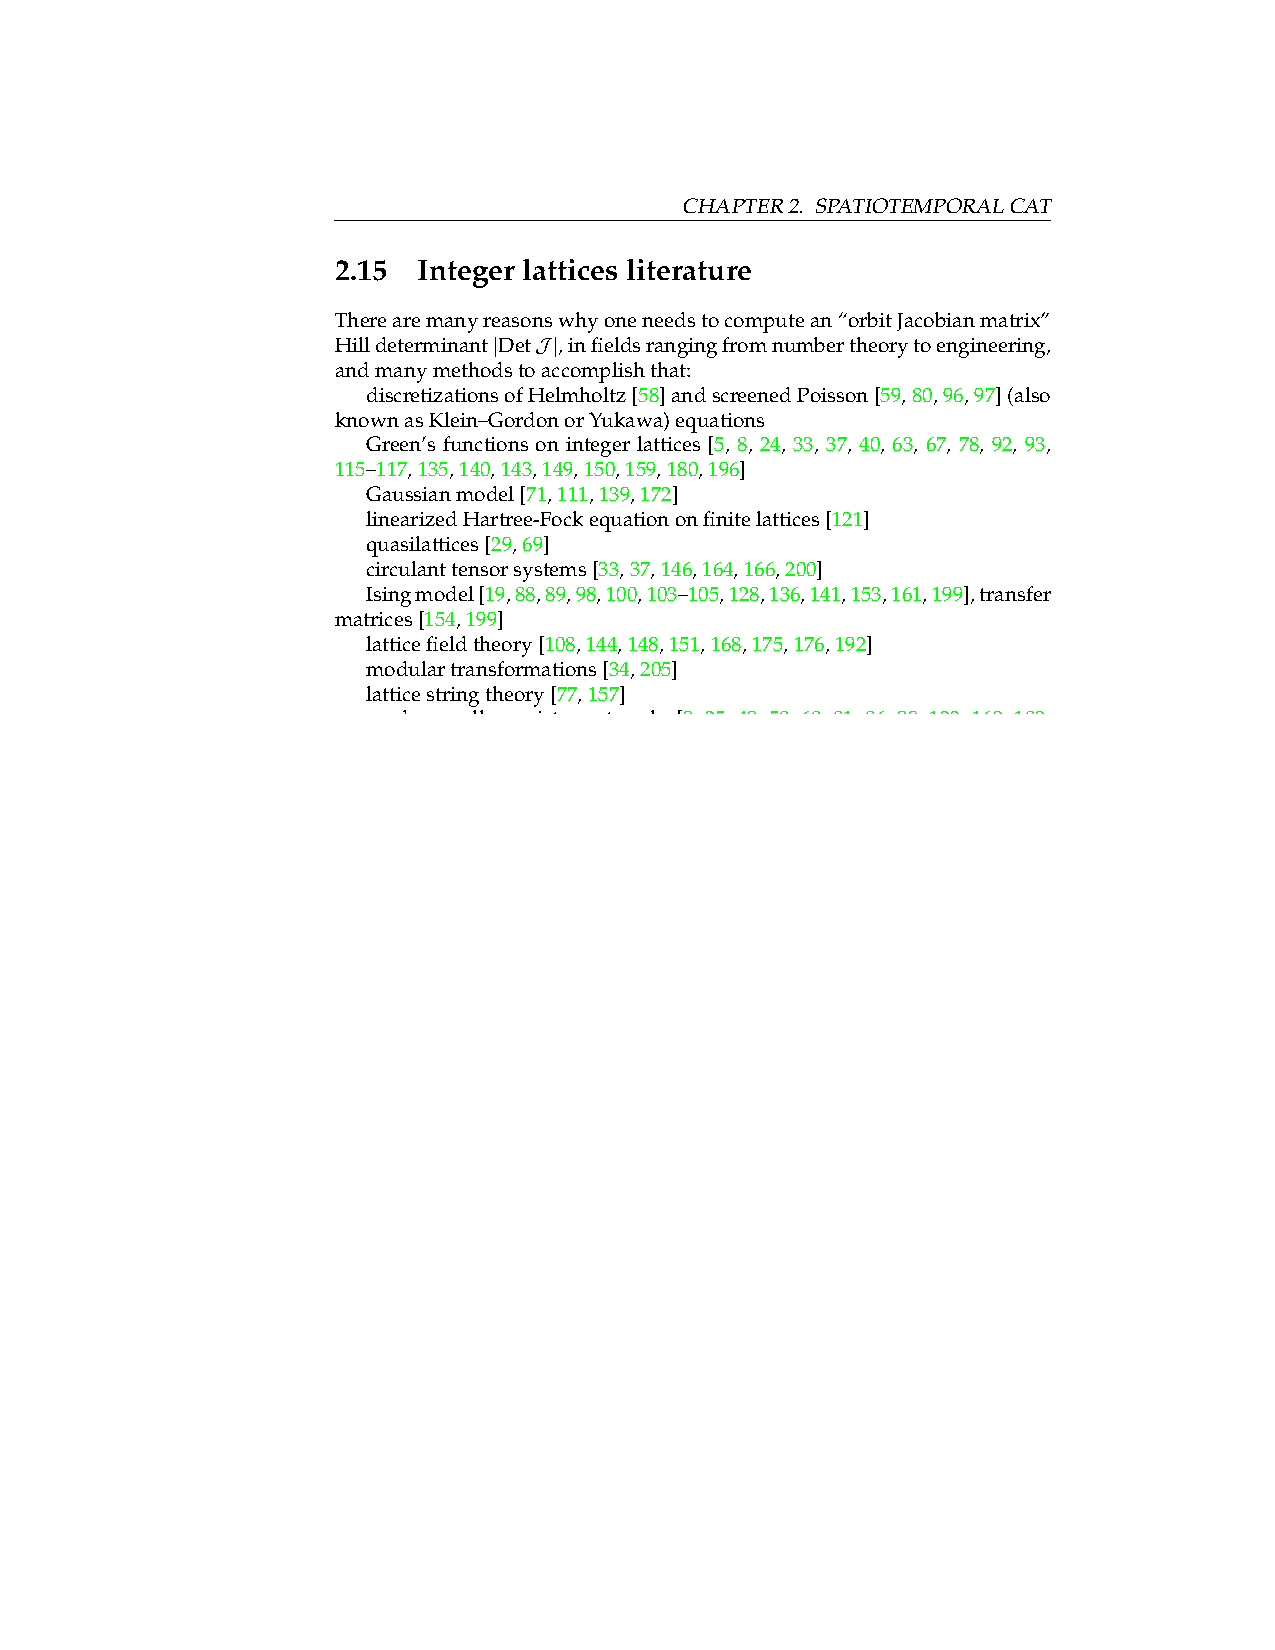
\includegraphics[width=0.90\textwidth]{../kittens/lattLitClip1}
\end{center}
\end{frame} %%%%%%%%%%%%%%%%%%%%%%%%%%%%%%%%%%%%%%%%%%%%%%

\begin{frame}{Zetastan : lost, but not alone}
\begin{center}
\hfill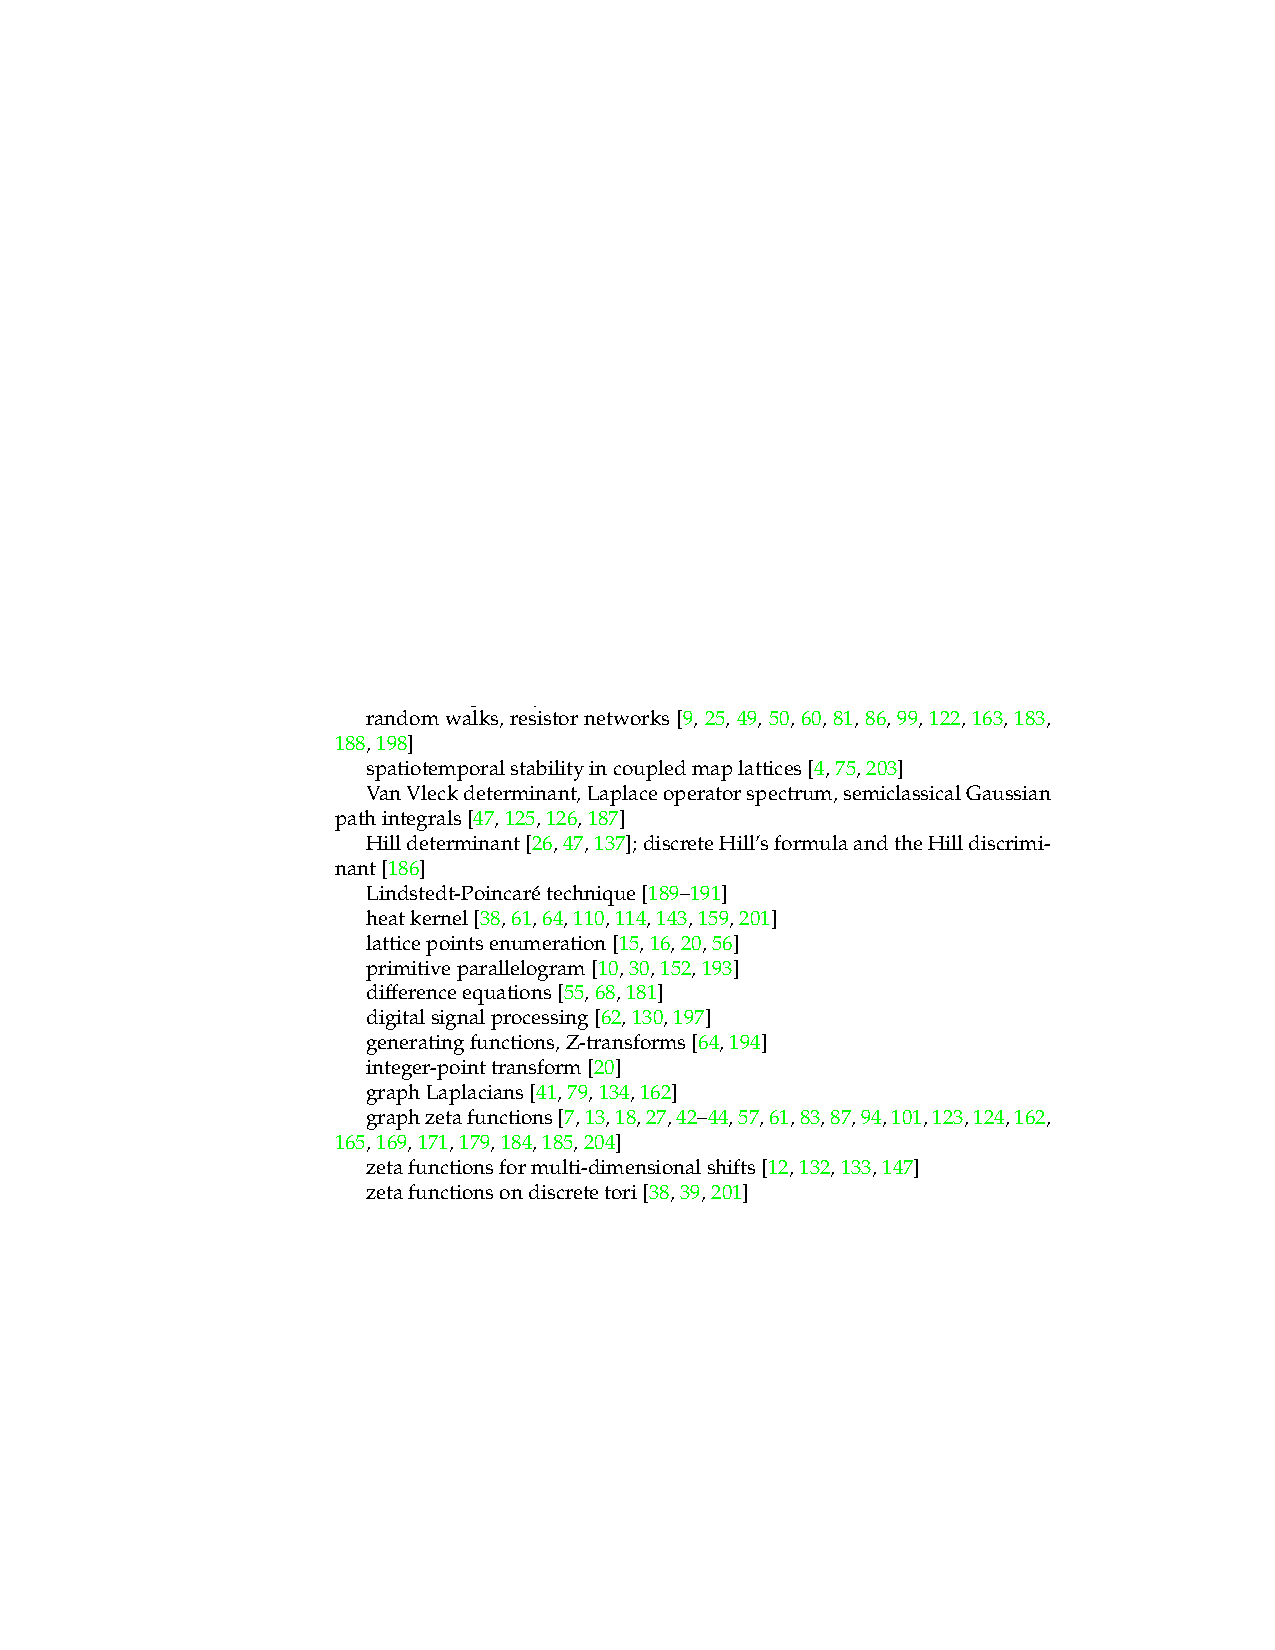
\includegraphics[width=0.90\textwidth]{../kittens/lattLitClip2}
\end{center}
\end{frame} %%%%%%%%%%%%%%%%%%%%%%%%%%%%%%%%%%%%%%%%%%%%%%

\begin{frame}{side remark to experts}
    \begin{block}{SL$_2(\integers)$ unimodular invariance of square lattice}
\begin{center}
  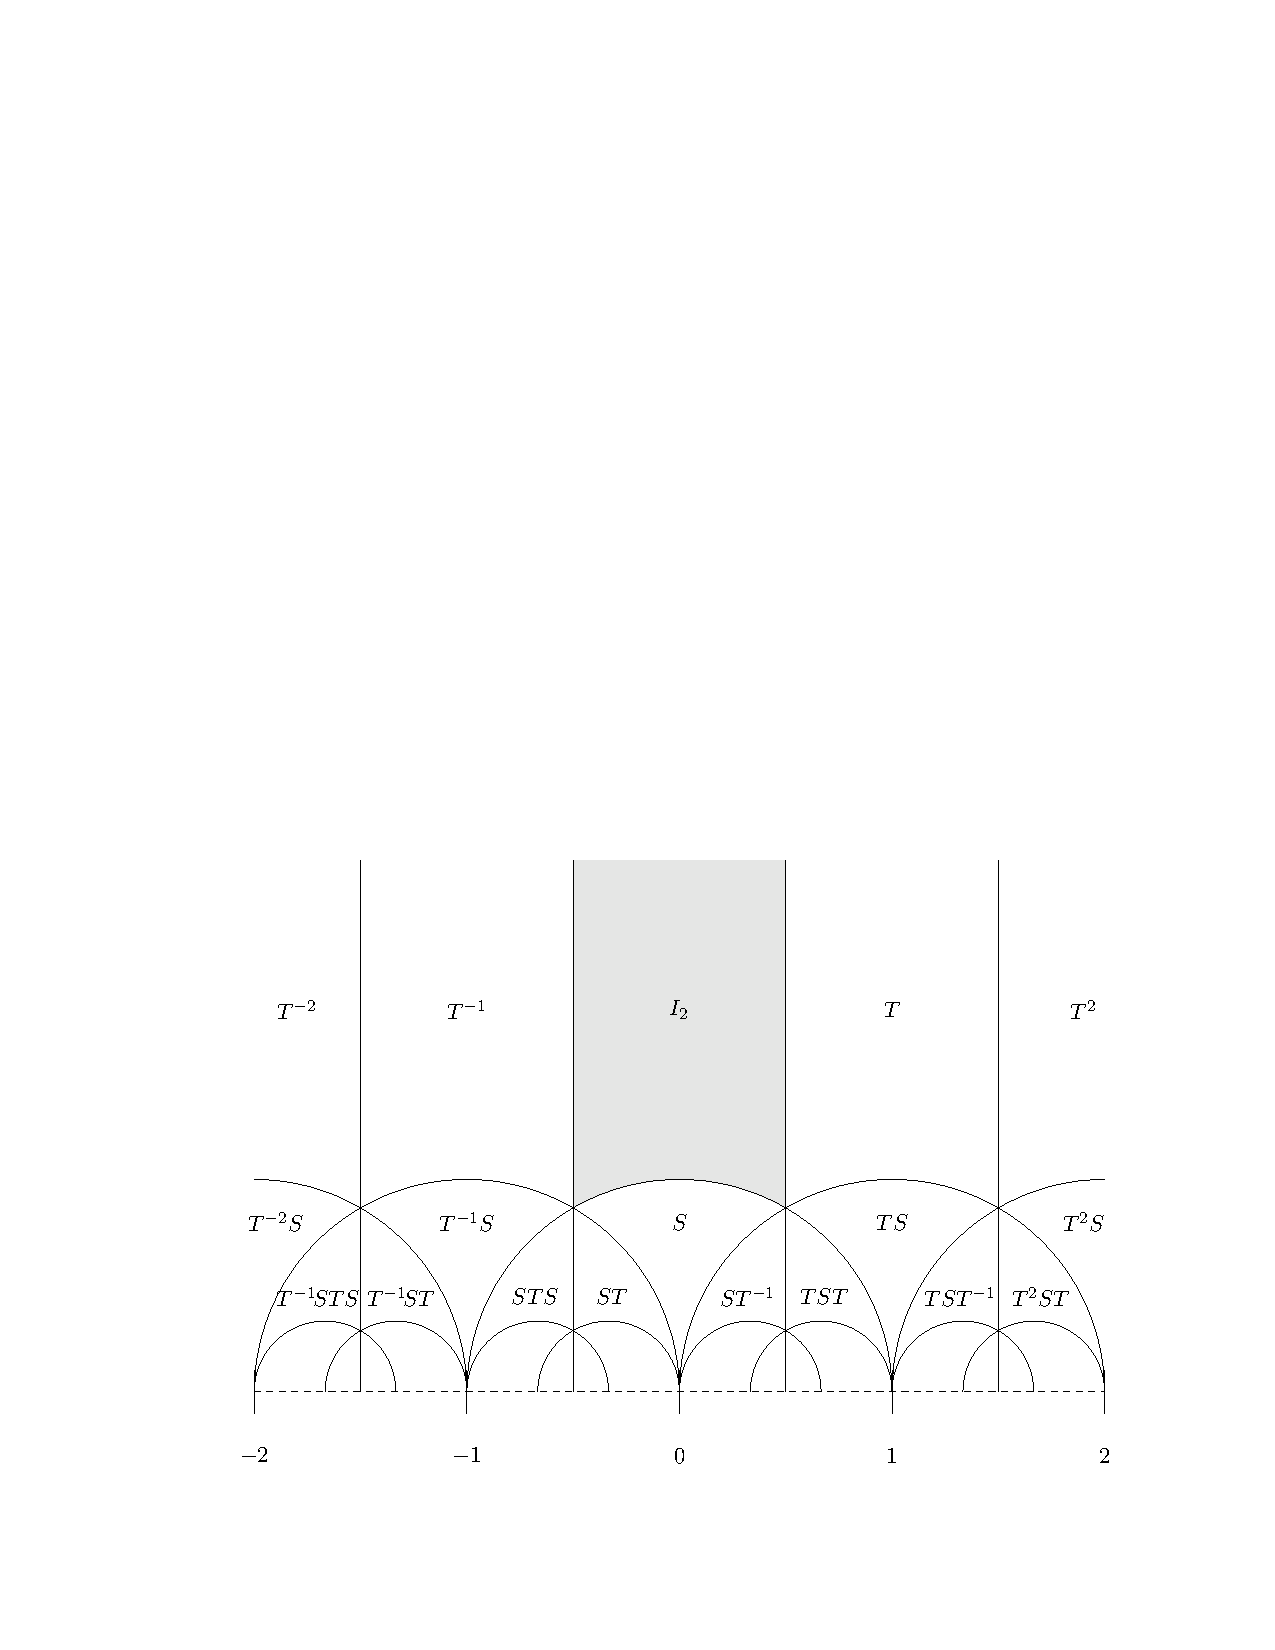
\includegraphics[width=0.65\textwidth]{ConradSL2Z}
\end{center}
Action on the complex upper half-plane by linear
fractional transformations $T$ and $S$.
~~~~~(figure: Keith Conrad)
    \end{block}
\bigskip

infinitely many `Bravais cells' for the same lattice
\end{frame} %%%%%%%%%%%%%%%%%%%%%%%%%%%%%%%%%%%%%%%%%%%%%%

\begin{frame}{but, is this}
\vfill
\begin{center}
{\huge chaos?}
\end{center}
\vfill
yes, short tiles are exponentially good `shadows' of the larger ones,
so can attain any desired accuracy
\end{frame} %%%%%%%%%%%%%%%%%%%%%%%%%%%%%%%%%%%%%%%%%%%%%%

\begin{frame}{is \catlatt\ `chaotic'?}
in time-evolving deterministic chaos any chaotic trajectory is
{\color{blue}shadowed by shorter \po s}
\bigskip

in \spt\ chaos, any unstable lattice state is {\color{blue}shadowed by
smaller \twots}
(Gutkin \etal\footfullcite{GutOsi15}${}^{,}${}\footfullcite{GHJSC16})

\vfill

next figure : code the \Mm\ symbol \brick\  $\ssp_{n\zeit}$ at the
lattice site $n\zeit$ with (color) alphabet
\[
\Ssym{t\ell} \in \A=\{\underline{1},0,1,2,\cdots\}=
\{%
{\color{red}red},
{\color{green}green},
{\color{blue}blue},
{\color{yellow}yellow},\cdots%
\}
\]

\end{frame} %%%%%%%%%%%%%%%%%%%%%%%%%%%%%%%%%%%%%%%%%%%%%%

\begin{frame}{shadowing, symbolic dynamics space}
\begin{center}
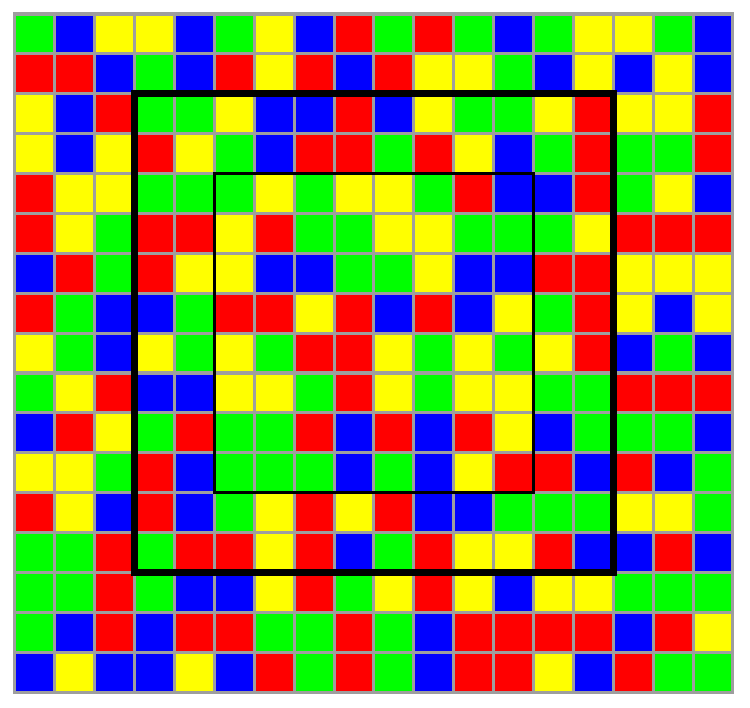
\includegraphics[width=0.45\textwidth]
{AKSs7colrBorderM1}\hspace{0.7cm}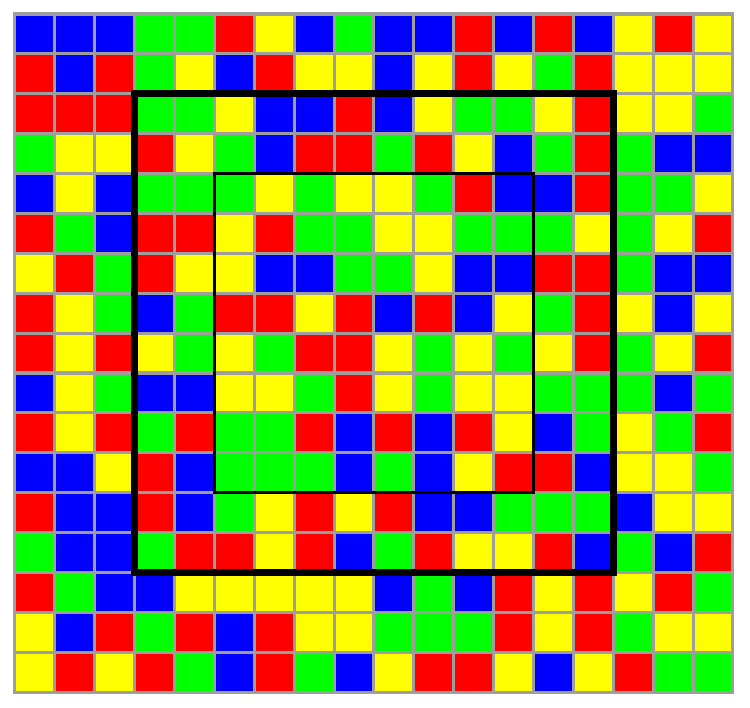
\includegraphics[width=0.45\textwidth]
{AKSs7colrBorderM2}
\end{center}
2d symbolic representation $\Mm_j$ of two lattice states $\Xx_j$
shadowing each other within the shared
\brick\ $\Mm_{\R}$ %=\Mm_{\R_{0}} \cup \Mm_{\R_{1}}$ (blue)

\begin{itemize}
  \item border $\R$ (thick black) %, interior $\R_{0}$ (thin black)
  \item symbols outside \R\ differ
\end{itemize}
\vfill
$s=7/2$    \hfill                          Adrien Saremi 2017
%\label{fig:AKScloseActSymb}
%%%%%%%%%%%%%%%%%%%%%%%%%%%%%%%%%%%%%%%%%%%%%%%%%%%%%%%%%%%%%%%%%%%%%%%
\end{frame} %%%%%%%%%%%%%%%%%%%%%%%%%%%%%%%%%%%%%%%%%%%%%%

\begin{frame}{shadowing} %, \statesp}
%%%%%%%%%blogCats \label{fig:AKSs7dist} %%%%%%%%%%%%%%%%%%%%%%%%%%%%%
\begin{center}
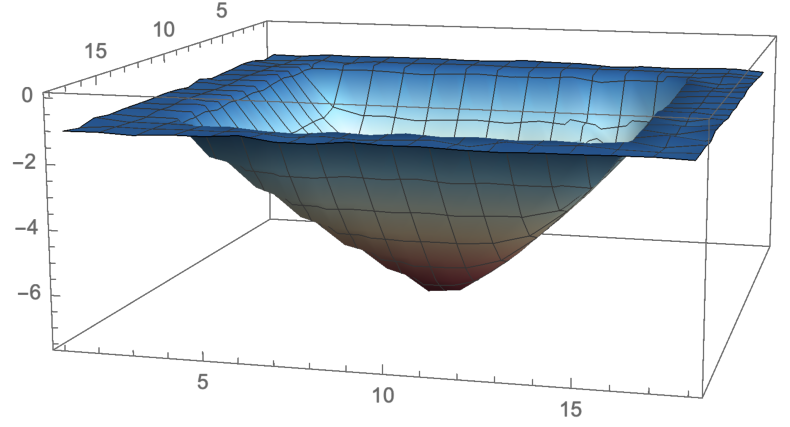
\includegraphics[width=0.65\textwidth]
{HL18ShadowingDistanceAverageLog3D}
\end{center}

\bigskip

the logarithm of the average of the absolute value of site-wise distance
\[
\ln|\ssp_{2,z}-\ssp_{1,z}|
\]
averaged over 250 solution pairs
\medskip

note the exponential falloff of the distance away from the center of the
shared \brick\ $\R$ %=\R_{0} \cup \R_{1}$.
\medskip

$\Rightarrow$ within the interior of the shared \brick,

\hfill \textcolor{blue}{shadowing is exponentially close}
\end{frame} %%%%%%%%%%%%%%%%%%%%%%%%%%%%%%%%%%%%%%%%%%%%%%

\begin{frame}{our song of chaos has been sang -- what next ?}
\begin{enumerate}
              \item \textcolor{gray}{\small
%what this is about
%              \item
coin toss
              \item
kicked rotor
              \item
\catlatt
                  }
              \item {\Large
bye bye, dynamics
%                  }\textcolor{gray}{\small
%              \item
%bye bye, dynamics
                    }
            \end{enumerate}
\end{frame} %%%%%%%%%%%%%%%%%%%%%%%%%%%%%%%%%%%%%%%%%%%%%%


\section[bye bye, dynamics]
 {bye bye, dynamics}
\label{s:byeDynamics}

\begin{frame}{the goal was}
\vfill

\begin{center}
{\Large build
\\
a chaotic field theory
\medskip

from
\\
the simplest chaotic blocks}
\end{center}

\vfill
using
\begin{itemize}
  \item
\textcolor{blue}{time invariance}
  \item
\textcolor{blue}{space invariance}
\end{itemize}
 of the defining partial differential equations
\end{frame} %%%%%%%%%%%%%%%%%%%%%%%%%%%%%%%%%%%%%%%%%%%%%%

\begin{frame}{take-home :   }
\begin{center}
            \begin{minipage}[c]{0.40\textwidth}\begin{center}
{\color{purple}harmonic} field theory
\bigskip

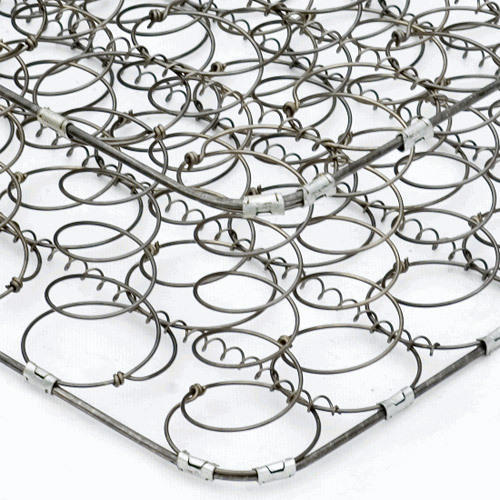
\includegraphics[width=0.85\textwidth]{mattressSpring}\\
{\color{blue}tight-binding} model
            \end{center}\end{minipage}
            \hspace{2ex}
            \begin{minipage}[c]{0.46\textwidth}\begin{center}
{\color{purple}chaotic} field theory\\
\bigskip
\bigskip
\bigskip

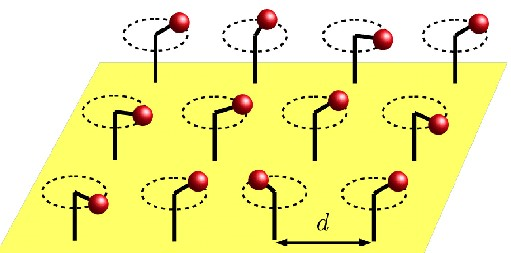
\includegraphics[width=1.0\textwidth]{flagellum1}\\
\bigskip

Euclidean {\color{blue}Klein-Gordon}
            \end{center}\end{minipage}
\end{center}
\end{frame}%%%%%%%%%%%%%%%%%%%%%%%%%%%%%%%%%%%%%%%%%%%%%%

\begin{frame}{what have we learned about spatiotemporal chaos?}
%\begin{center}
%\hfill
\includegraphics[width=0.55\textwidth]{spatiotempCat}
\catlatt\hfill
\includegraphics[width=0.55\textwidth]{DawnBishopCats}
%\end{center}
\end{frame} %%%%%%%%%%%%%%%%%%%%%%%%%%%%%%%%%%%%%%%%%%%%%%


\begin{frame}{insight 1 : how is turbulence described?}
\begin{block}{not by the evolution of an initial state}
exponentially unstable system have finite (Lyapunov) time and
space prediction horizons
\end{block}
but
\bigskip

\begin{block}{by enumeration of admissible field configurations}
and their natural weights
\end{block}
\end{frame} %%%%%%%%%%%%%%%%%%%%%%%%%%%%%%%%%%%%%%%%%%%%%%

\begin{frame}{insight 2 : symbolic dynamics for turbulent flows}
applies to
all PDEs with \textcolor{red}{$d$} translational symmetries

\bigskip

a $d$\dmn\ spatiotemporal field configuration
\[
\{\ssp_{z}\} = \{\ssp_{z},  z\in \integers^{d}  \}
\]
is labelled by a \textcolor{red}{$d$\dmn} {spatiotemporal
{\brick}} of symbols
\[
\{\m_{z}\} = \{\m_{z}, z\in \integers^{d}\}
\,,
\]

\bigskip

rather than a \textcolor{red}{single} temporal symbol sequence

\bigskip

(as is done when describing a small coupled few-``body'' system, or a
small computational domain).
\end{frame} %%%%%%%%%%%%%%%%%%%%%%%%%%%%%%%%%%%%%%%%%%%%%%


\begin{frame}{insight 3 : description of turbulence by \twots}
\begin{block}{1 time, 0 space dimensions}
a {\statesp} point is {\em periodic} if its orbit returns to itself
after a finite time \period{}; such orbit tiles the time axis
by infinitely many repeats
\end{block}

\bigskip

\begin{block}{1 time, $d$-1 space dimensions}
 a {\statesp} point is {\em spatiotemporally periodic} if
it belongs to \\ an invariant $d$-torus ${\R}$,\\
\ie, a \brick\ $\Mm_{\R}$ that
tiles the lattice state  $\Mm$, \\
with period $\ell_j$ in $j$th lattice direction
\end{block}
\end{frame} %%%%%%%%%%%%%%%%%%%%%%%%%%%%%%%%%%%%%%%%%%%%%%

\begin{frame}{bye bye, dynamics}
\begin{enumerate}
              \item
goal : describe states of turbulence in infinite spatiatemporal domains
              \item
theory : classify, enuremate all spatiotemporal tilings
              \item
example : \catlatt, the simplest model of ``turbulence''
\end{enumerate}

\vfill

there is no more time

\medskip

there is only enumeration of admissible spacetime field configurations
\end{frame} %%%%%%%%%%%%%%%%%%%%%%%%%%%%%%%%%%%%%%%%%%%%%%


\begin{frame}{Verbrechen des Jahrhunderts : das Ende der Zeit}
\begin{center}
\textcolor{red}{{\huge {\huge die Zeit ist tot} !}}
\end{center}
\end{frame} %%%%%%%%%%%%%%%%%%%%%%%%%%%%%%%%%%%%%%%%%%%%%%

\begin{frame}{crime of the century : this the end of time}
\begin{center}
\textcolor{red}{{\huge time is dead !}}
\end{center}
\end{frame} %%%%%%%%%%%%%%%%%%%%%%%%%%%%%%%%%%%%%%%%%%%%%%

\begin{frame}{in future there will be no future}
\begin{center}
{\huge goodbye}
\end{center}

\vfill

to long time and/or space integrators

\medskip

\hfill they never worked and could never work
\end{frame} %%%%%%%%%%%%%%%%%%%%%%%%%%%%%%%%%%%%%%%%%%%%%%

\begin{frame}{insight 4 : can compute `all' solutions}
Bernoulliland - rough initial guesses converge
\begin{center}
\hfill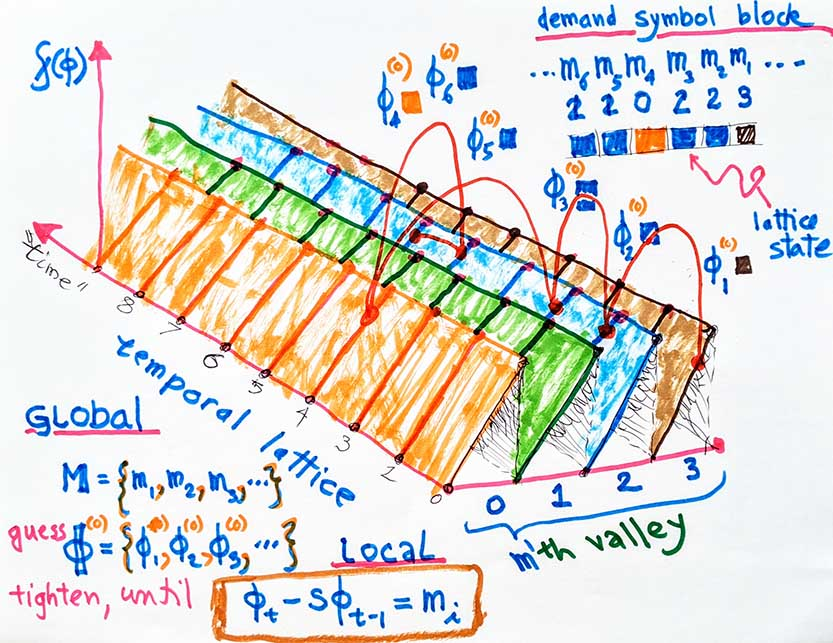
\includegraphics[width=0.85\textwidth]{PC200923Bernoulli2}
\end{center}
no exponential instabilities
\end{frame} %%%%%%%%%%%%%%%%%%%%%%%%%%%%%%%%%%%%%%%%%%%%%%

\begin{frame}{miaw}
\vfill
the stage is set for the quantum field theory of \catlatt, the details of
which we leave to our always trustworthy
friends Jon Keating and Marcos Saraceno
\end{frame} %%%%%%%%%%%%%%%%%%%%%%%%%%%%%%%%%%%%%%%%%%%%%%


%%% #######################################



\end{document}
